\documentclass[]{article}

\usepackage[utf8]{inputenc}
\usepackage[english]{babel}

\usepackage{amsmath,amsthm,amsfonts,amssymb,bm}
\usepackage{mathtools}

\usepackage[linesnumbered,lined,ruled,vlined]{algorithm2e}
\SetKwInput{KwInput}{Inputs}
\SetKwProg{Func}{Function}{}{end}

\usepackage{graphicx}
\usepackage{hyperref}
\hypersetup{colorlinks=false, hidelinks}

\usepackage[authoryear, round]{natbib}

%!TEX root = main.tex
% Generic macro definitions for a number of math operations.
% Version 2.0, last updated 10.05.2022.
%
% To use this macro you need packages: amsmath, amssymb, bm, mathtools
% 
% Zheng Zhao @ 2019
% zz@zabemon.com
%
% License: Creativice Commons Attribution 4.0 International (CC BY 4.0)
%

% Adaptive bold math font command
\newcommand{\cu}[1]{
	\ifcat\noexpand#1\relax
	\bm{#1}
	\else
	\mathbf{#1}
	\fi
}

\newcommand{\tash}[2]{\frac{\partial #1}{\partial #2}}
\newcommand{\tashh}[3]{\frac{\partial^2 #1}{\partial #2 \, \partial #3}}

% Slightly smaller spacing than a pure mathop
\newcommand{\diff}{\mathop{}\!\mathrm{d}}

% Complex
\newcommand{\imag}{\mathrm{i}}

% Exponential
\newcommand{\expp}{\mathrm{e}}

% \mid used in condition in probability e.g., E[x \mid y]
\newcommand{\cond}{{\;|\;}}
\newcommand{\condbig}{{\;\big|\;}}
\newcommand{\condBig}{{\;\Big|\;}}
\newcommand{\condbigg}{{\;\bigg|\;}}
\newcommand{\condBigg}{{\;\Bigg|\;}}

\let\sup\relax
\let\inf\relax
\let\lim\relax
\DeclareMathOperator*{\argmin}{arg\,min\,}  % Argmin
\DeclareMathOperator*{\argmax}{arg\,max\,}  % Argmax
\DeclareMathOperator*{\sup}{sup\,}  % sup better spacing
\DeclareMathOperator*{\inf}{inf\,}  % inf
\DeclareMathOperator*{\lim}{lim\,}  % inf
\DeclareMathOperator*{\oprepeat}{\cdots}  % repeat operation

\newcommand{\sgn}{\operatorname{sgn}}           % sign function

\newcommand{\expecsym}{\operatorname{\mathbb{E}}}     % Expec
\newcommand{\covsym}{\operatorname{Cov}}     % Covariance
\newcommand{\varrsym}{\operatorname{Var}}     % Variance
\newcommand{\diagsym}{\operatorname{diag}}     % Diagonal matrix
\newcommand{\tracesym}{\operatorname{tr}}           % Trace

% Two problems for E, Cov, Var etc. with brackets
% 1. \operatorname does not give space for bracket, thus we need to manually add \, after E. If \left\right is used then no need to add space.
% 2. \left\right does not give correct vertical spacing. The brackets will be shifted down slightly.
% Solution is to use \left\right when it is inevitable.
% Use \expec when you do not want auto-height
% Use \expec* when you want auto-height
% Use \expecsym when you want to fully define the behaviour, which only gives the E symbol wihout brackets. 
\let\expec\relax
\let\cov\relax
\let\varr\relax
\let\diag\relax
\let\trace\relax

\makeatletter
% E [ ]
\newcommand{\expec}{\@ifstar{\@expecauto}{\@expecnoauto}}
\newcommand{\@expecauto}[1]{\expecsym \left[ #1 \right]}
\newcommand{\@expecnoauto}[1]{\expecsym [#1]}
\newcommand{\expecbig}[1]{\expecsym \bigl[ #1 \bigr]}
\newcommand{\expecBig}[1]{\expecsym \Bigl[ #1 \Bigr]}
\newcommand{\expecbigg}[1]{\expecsym \biggl[ #1 \biggr]}
\newcommand{\expecBigg}[1]{\expecsym \Biggl[ #1 \Biggr]}


% Cov [ ]
\newcommand{\cov}{\@ifstar{\@covauto}{\@covnoauto}}
\newcommand{\@covauto}[1]{\covsym \left[ #1 \right]}
\newcommand{\@covnoauto}[1]{\covsym [#1]}
\newcommand{\covbig}[1]{\covsym \bigl[ #1 \bigr]}
\newcommand{\covBig}[1]{\covsym \Bigl[ #1 \Bigr]}
\newcommand{\covbigg}[1]{\covsym \biggl[ #1 \biggr]}
\newcommand{\covBigg}[1]{\covsym \Biggl[ #1 \Biggr]}

% Var [ ]
\newcommand{\varr}{\@ifstar{\@varrauto}{\@varrnoauto}}
\newcommand{\@varrauto}[1]{\varrsym \left[ #1 \right]}
\newcommand{\@varrnoauto}[1]{\varrsym [#1]}
\newcommand{\varrbig}[1]{\varrsym \bigl[ #1 \bigr]}
\newcommand{\varrBig}[1]{\varrsym \Bigl[ #1 \Bigr]}
\newcommand{\varrbigg}[1]{\varrsym \biggl[ #1 \biggr]}
\newcommand{\varrBigg}[1]{\varrsym \Biggl[ #1 \Biggr]}

% Diag ( )
\newcommand{\diag}{\@ifstar{\@diagauto}{\@diagnoauto}}
\newcommand{\@diagauto}[1]{\diagsym \left( #1 \right)}
\newcommand{\@diagnoauto}[1]{\diagsym (#1)}
\newcommand{\diagbig}[1]{\diagsym \bigl( #1 \bigr)}
\newcommand{\diagBig}[1]{\diagsym \Bigl( #1 \Bigr)}
\newcommand{\diagbigg}[1]{\diagsym \biggl( #1 \biggr)}
\newcommand{\diagBigg}[1]{\diagsym \Biggl( #1 \Biggr)}

% tr ( )
\newcommand{\trace}{\@ifstar{\@traceauto}{\@tracenoauto}}
\newcommand{\@traceauto}[1]{\tracesym \left( #1 \right)}
\newcommand{\@tracenoauto}[1]{\tracesym (#1)}
\newcommand{\tracebig}[1]{\tracesym \bigl( #1 \bigr)}
\newcommand{\traceBig}[1]{\tracesym \Bigl( #1 \Bigr)}
\newcommand{\tracebigg}[1]{\tracesym \biggl( #1 \biggr)}
\newcommand{\traceBigg}[1]{\tracesym \Biggl( #1 \Biggr)}
\makeatother

\newcommand{\A}{\mathcal{A}}           % Generator
\newcommand{\Am}{\overline{\mathcal{A}}}           % Generator

% Transpose symbol using (DIN) EN ISO 80000-2:2013 standard
\newcommand*{\trans}{{\mkern-1.5mu\mathsf{T}}}
\newcommand*{\conjtrans}{\mathsf{H}}

\newcommand*{\T}{\mathbb{T}} % Set of temporal varialbes
\newcommand*{\R}{\mathbb{R}} % Set of real numbers
\newcommand*{\Q}{\mathbb{Q}} % Set of rational numbers
\newcommand*{\N}{\mathbb{N}} % Set of natural numbers
\newcommand*{\Z}{\mathbb{Z}} % Set of integers

\newcommand*{\BB}{\mathcal{B}} % Borel sigma-algebra
\newcommand*{\FF}{\mathcal{F}} % Sigma-algebra
\newcommand*{\PP}{\mathbb{P}} % Probability measure
\newcommand*{\GP}{\mathrm{GP}} % GP

\newcommand{\mineig}{\lambda_{\mathrm{min}}}
\newcommand{\maxeig}{\lambda_{\mathrm{max}}}

% Norm and inner product
%% use \norm* to enable auto-height

%% Some notes on these paired delimiters:
%% It is argued that there should be no space between operator and delimiter, but this might not be suitable in some cases. Indeed log(x) should have no space between log and (, but log |x| with a mathop{} spacing looks absolutely much prettier than log|x| because here |x| is an argument. Think, shouldn't it be log(|x|) in full expansion, and we ignored () with spacing?
%% See discussion in https://tex.stackexchange.com/questions/461806/missing-space-with-declarepaireddelimiter
%
\let\norm\relax
\DeclarePairedDelimiter{\normbracket}{\lVert}{\rVert}
\newcommand{\norm}{\normbracket}
\newcommand{\normbig}[1]{\big \lVert #1 \big \rVert}
\newcommand{\normBig}[1]{\Big \lVert #1 \Big\rVert}
\newcommand{\normbigg}[1]{\bigg \lVert #1 \bigg\rVert}
\newcommand{\normBigg}[1]{\Bigg \lVert #1 \Bigg\rVert}
%\makeatletter
%\newcommand{\norm}{\@ifstar{\@normnoauto}{\@normauto}}
%\newcommand{\@normauto}[1]{\left\lVert#1\right\rVert}
%\newcommand{\@normnoauto}[1]{\lVert#1\rVert}
%\makeatother

\let\innerp\relax
\DeclarePairedDelimiter{\innerpbracket}{\langle}{\rangle}
\newcommand{\innerp}{\innerpbracket}
%\makeatletter
%\newcommand{\innerp}{\@ifstar{\@inpnoautp}{\@inpauto}}
%\newcommand{\@inpauto}[2]{\left\langle#1, #2\right\rangle}
%\newcommand{\@inpnoautp}[2]{\left#1, #2\rangle}
%\makeatother

\let\abs\relax
\DeclarePairedDelimiter{\absbracket}{\lvert}{\rvert}
\newcommand{\abs}{\absbracket}
\newcommand{\absbig}[1]{\big \lvert #1 \big \rvert}
\newcommand{\absBig}[1]{\Big \lvert #1 \Big\rvert}
\newcommand{\absbigg}[1]{\bigg \lvert #1 \bigg\rvert}
\newcommand{\absBigg}[1]{\Bigg \lvert #1 \Bigg\rvert}
%\makeatletter
%\newcommand{\abs}{\@ifstar{\@absnoauto}{\@absauto}}
%\newcommand{\@absauto}[1]{\left\lvert#1\right\rvert}
%\newcommand{\@absnoauto}[1]{\lvert#1\rvert}
%\makeatother

% Some functions
\newcommand{\mBesselsec}{\operatorname{K}_\nu}
\newcommand{\jacob}{\operatorname{J}}
\newcommand{\hessian}{\operatorname{H}}

% Literals
\def\matern{Mat\'{e}rn }

% Theorem envs
% Dummy env for those sharing the same numbering system.
% If you would like to customise your environment numbering, you can define a command e.g., \thmnumcounter{section} in your main tex.
% If \thmnumcounter is undefined, it is assumed that you will deal with defining theorem lemma etc by yourself.
\makeatletter
\@ifundefined{thmenvcounter}{}
{%
	\newtheorem{envcounter}{EnvcounterDummy}[\thmenvcounter]
	\newtheorem{definition}[envcounter]{Definition}
	\newtheorem{theorem}[envcounter]{Theorem}
	\newtheorem{proposition}[envcounter]{Proposition}
	\newtheorem{lemma}[envcounter]{Lemma}
	\newtheorem{corollary}[envcounter]{Corollary}
	\newtheorem{remark}[envcounter]{Remark}
	\newtheorem{example}[envcounter]{Example}
	\newtheorem{exercise}[envcounter]{Exercise}
	\newtheorem{definition}[envcounter]{Definition}
	\newtheorem{algorithm}[envcounter]{Algorithm}
	\newtheorem{assumption}[envcounter]{Assumption}
}
\makeatother



\newtheorem{theorem}{Theorem}
\newtheorem{proposition}[theorem]{Proposition}
\newtheorem{definition}[theorem]{Definition}
\newtheorem{remark}[theorem]{Remark}
\newtheorem{example}[theorem]{Example}
\newtheorem{exercise}[theorem]{Exercise}

\begin{document}

\begin{titlepage}
	\let\newpage\relax
	
	\begin{center}
		\vspace*{0.1cm}
		
		\Large{\textbf{Lecture note: Gaussian processes}}
		
		\vspace{0.2em}
		
		\normalsize{in HT2022 Advanced Probabilistic Machine Learning}
		
		\vspace{1cm}
		
		Zheng Zhao\footnote{Contact: firstname.lastname@it.uu.se. To download the \LaTeX~source and companion codes of this lecture note, please visit \url{https://github.com/spdes/gp}.}
		
		\vspace{0.2em}
		
		Uppsala Universitet
		
		\vspace{0.2em}
		
		Last update: 20 September, 2022
	\end{center}
	
	\textbf{Target audience}: students with background, for example, machine learning, engineering, statistics, and physics.
	
	\textbf{Time}: Around 3 hours.
	
	\vspace{0.5cm}
\end{titlepage}

%\tableofcontents


\section{Introduction}
\label{sec:intro}
Let us start by considering an example function $X\colon [0, \infty) \to \R$ defined by
%
\begin{equation}
	X(t) = a \, t + b,
	\label{equ:example-gp-linear-cov}
\end{equation}
%
where $a$ and $b$ are some real parameters. Now that if we let $a \sim \mathrm{N}(m_a, v_a)$ and $b \sim \mathrm{N}(m_b, v_b)$ be two independent Normal random variables instead of fixed reals, $X$ then becomes a random variable as well. This $X$ is the basic object that we have studied in the previous lecture on Bayesian linear regression. Furthermore, we can view $X$ as a function-valued random variable, since whenever we draw a pair of samples from $\lbrace a, b\rbrace$ we obtain an affine function which is a sample from $X$; this is illustrated in Figure~\ref{fig:example-gp-cov-linear}.

The random variable $X$ in this example is a Gaussian process (GP), the definition of which we detail in the following section. 
%
\begin{figure}[h!]
	\centering
	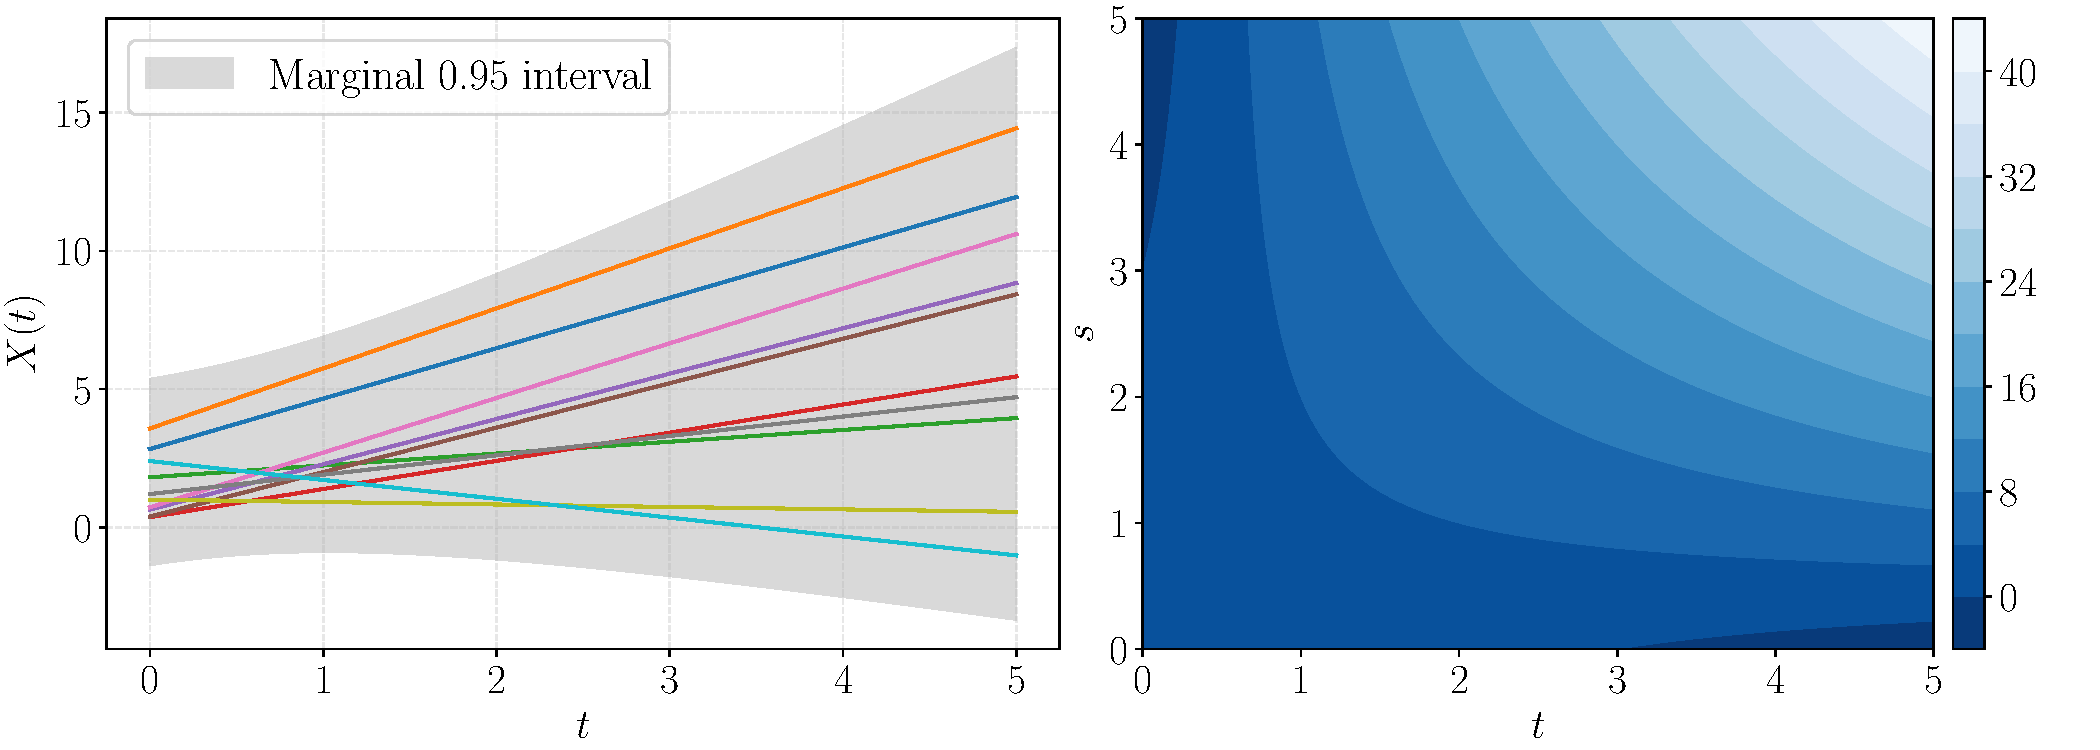
\includegraphics[width=.99\linewidth]{figs/example-gp-affine-sample-cov}
	\caption{Left: samples (in different colours) of $X$ in Equation~\eqref{equ:example-gp-linear-cov} are affine functions, where in this example we let $m_a = 1$, $v_a = 1$, $m_b = 2$, and $v_b = 3$. Right: contour plot of the covariance function of $X$.}
	\label{fig:example-gp-cov-linear}
\end{figure}

\section{Gaussian processes}
\label{sec:gp}
Indeed we can define GP as function-valued random variable following the heuristics in Introduction. Say, for example, if $X$ takes value in a Hilbert space of functions $H$ endowed with inner product $\innerp{\cdot, \cdot}$, then we say that $X$ is $H$-Gaussian if $\innerp{X, u}$ is Gaussian in $\R$ for all $u \in H$, and you perhaps very often see ``GP is an infinite-dimensional prior'' in many textbooks/lecture notes. However, the precise definition of GP in this routine requires to introduce infinite-dimensional Gaussian measures~\citep[see, e.g.,][]{Kuo1975} which is not within the scope of this lecture note. Therefore, we give a definition of GP in terms of finite-dimensional Gaussian distributions as follows, since we can view stochastic process as a collection of random variables as well (i.e., $X\coloneqq \lbrace X(t) \colon t\geq 0\rbrace$).

\begin{definition}[Gaussian process]
	\label{def:gp}
	A stochastic process $X\coloneqq \lbrace X(t) \in \R \colon t\geq 0\rbrace$ is said to be a Gaussian process on $[0, \infty)$, if for every $T \geq 1$ and reals $t_1<t_2<\cdots <t_T \in [0, \infty)$, the random variables $X(t_1), X(t_2), \ldots, X(t_T)$ are jointly Normal distributed~\citep{Karatzas1991}.
\end{definition}

Since the distribution of Normal random variables are determined by their means and covariances, we usually translate Definition~\ref{def:gp} by a shorthand~\citep[commonly seen in the statistical machine learning community, see, e.g.,][]{Rasmussen2006}
%
\begin{equation}
	X(t) \sim \GP\bigl(m(t), C(t, s)\bigr),
	\label{equ:gp-notation}
\end{equation}
%
where $m$ and $C$ stand for the mean and covariance functions of $X$, respectively, and they are defined by
%
\begin{equation*}
	\begin{split}
		m(t) &\coloneqq \expec{X(t)}, \\
		C(t, s) &\coloneqq \cov{X(t), X(s)},
	\end{split}
\end{equation*}
for all $t, s$. The mean and covariance functions also determine the probabilistic properties of $X$, such as continuity, volatility, and stationarity.

Now let us use notation $\mathrm{N}(x_{1:T} \cond m_{1:T}, C_{1:T})$ to denote the (multivariate) Normal probability density function (PDF) of $X_{1:T} \coloneqq [ X(t_1), X(t_2), \ldots, X(t_T) ] \allowbreak\in\R^T$ with its mean vector $m_{1:T} \in \R^T$ and covariance matrix (also known as the Gram matrix or kernel matrix) $C_{1:T} \in \R^{T\times T}$. Definition~\ref{def:gp} or Equation~\eqref{equ:gp-notation} \emph{essentially} means that  
%
\begin{equation}
	\begin{split}
		X_{1:T} &\sim 
		\mathrm{N}\left( 
		\begin{bmatrix}
			x_1 \\
			x_2 \\
			\vdots \\
			x_T
		\end{bmatrix} \condBigg
		\begin{bmatrix}
			m(t_1) \\
			m(t_2) \\
			\vdots \\
			m(t_T)
		\end{bmatrix}, 
		\begin{bmatrix}
			C(t_1, t_1) & C(t_1, t_2) & \cdots & C(t_1, t_T) \\
			C(t_2, t_1) & C(t_2, t_2) & \cdots & C(t_2, t_T) \\
			\vdots      & \vdots      &\ddots  & \vdots \\
			C(t_T, t_1) & C(t_T, t_2) & \cdots & C(t_T, t_T)
		\end{bmatrix}
		\right) \\
		&\coloneqq \mathrm{N}(x_{1:T} \cond m_{1:T}, C_{1:T}).
	\end{split}
	\label{equ:gp-pdf}
\end{equation}
%
Please note the emphasised ``essentially''. This warns that one should not take Definition~\ref{def:gp} and the multivariate Normal PDF representation of GP equivalent, because the PDF in Equation~\eqref{equ:gp-pdf} is well-defined only if the covariance matrix is positive definite. There is a plenty of counterexamples whose GP covariance matrices are not positive definite. For instance, let $X_0 \sim \mathrm{N}(0, 1)$ be a standard Gaussian and define $X(t) = X_0$ for all $t$. By Definition~\ref{def:gp}, this process $X$ is a GP, however, the covariance matrix of $X$ at any times $t_1, t_1, \ldots, t_T$ is an all-one matrix which is singular, hence, this GP $X$ does not have a PDF alike Equation~\eqref{equ:gp-pdf}. 

We can also define GP in terms of characteristic function. More precisely, we say that $X$ is a GP if for any $T\geq 1$ and times $t_1, t_2, \ldots, t_T$, the joint characteristic function $\phi_{X_{1:T}}$ of $X_{1:T}$ at these times follows
%
\begin{equation}
	\begin{split}
		\phi_{X_{1:T}}(z_{1:T}) &\coloneqq \expecbig{\exp(\imag \, z_{1:T}^\trans \, X_{1:T})}\\
		&= \exp\Biggl(\imag \sum^T_{k=1} m(t_k) \, z_k - \frac{1}{2} \sum^T_{j,k=1} C(t_j, t_k) \, z_j \, z_k \Biggr)  \\
		&= \exp \Bigl( \imag \, z_{1:T}^\trans \, m_{1:T} - \frac{1}{2} \, C_{1:T} \, z_{1:T} \Bigr).
	\end{split}
	\label{equ:gp-characteristic-func}
\end{equation}
%
The definition using the equation above is equivalent to Definition~\ref{def:gp}, moreover, the covariance matrix $C_{1:T}$ needs not to be positive definite. The characteristic function is mainly useful in analysis, for example, to show the distribution of a limit of random variables, we can conveniently show the limit of the characteristic function of the random variable in the sequence, thanks to the dominated convergence theorem.

\subsection{Example GPs}

For the sake of pedagogy, we exemplify and plot a few commonly seen GPs whose mean and covariance functions are explicitly given.

\begin{example}[Affine GP]
	\label{example:affine-gp}
	Recall the GP $X$ defined in Equation~\eqref{equ:example-gp-linear-cov}. By its definition, we find that its mean and covariance functions are 
	\begin{equation}
		\begin{split}
			m(t) &= m_a \, t + m_b, \\
			C(t, s) &= \cov{(a \, t + b), (a \, s + b)} \\
			&= v_a \, t \, s + v_b.
			\label{equ:affine-gp-mean-cov}
		\end{split}
	\end{equation}
	The samples and covariance matrix of this GP are plotted in Figure~\ref{fig:example-gp-cov-linear}.
\end{example}

\begin{example}[(Fractional) Brownian motion]
	Brownian motion (also known as Wiener process) is a fundamental stochastic process defined from independent Normal increments~\citep[see, e.g.,][for the precise definition]{Karatzas1991}. Its definition implies that it is a GP following the mean and covariance functions given by
	%
	\begin{equation*}
		\begin{split}
			m(t) &= 0,\\
			C(t, s) &= \min(t, s).
		\end{split}
	\end{equation*}
	%
	The sample path of a Brownian motion is rough, and the rough means that the path is almost surely non-differentiable and is H\"{o}lder continuous of degree less than $0.5$. To generalise Brownian motion with any degree of H\"{o}lder continuity, we use the fractional Brownian motion, the covariance function of which is given by
	%
	\begin{equation*}
		C(t, s; r) = 0.5 \, (\abs{t}^{2 \, r} + \abs{s}^{2 \, r} - \abs{t - s}^{2 \, r}),
	\end{equation*}
	%
	where $r \in (0, 1)$ is the parameter that controls the continuity. When $r=0.5$, the fractional Brownian motion reduces to a standard Brownian motion. Samples and covariance matrices of the fractional Brownian motion with $r=0.5$ and $0.9$ are shown in Figure~\ref{fig:fBM}.\footnote{Colourbars from now on are omitted for aesthetics, please compared to Figure~\ref{fig:example-gp-cov-linear} or generate the figure with colourbar by yourself from the companion codes.}
	%
	\begin{figure}[h!]
		\centering
		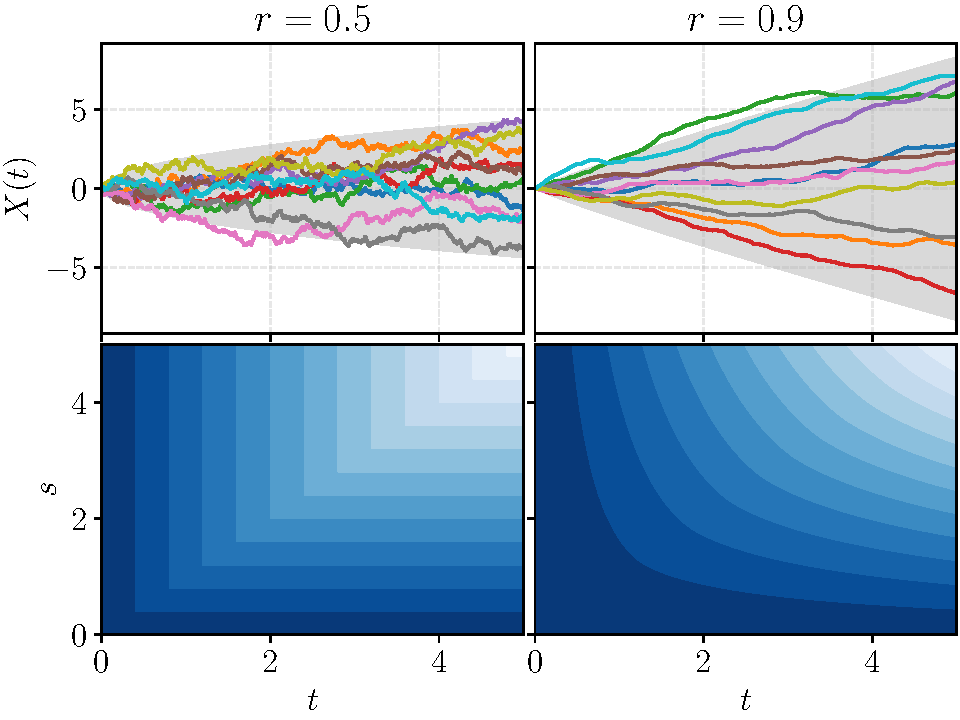
\includegraphics[width=.8\linewidth]{figs/sample-cov-fbm}
		\caption{Samples (top) and covariance matrices (bottom) of the standard Brownian motion (left) and a fractional Brownian motion with $r=0.9$ (right).}
		\label{fig:fBM}
	\end{figure}
\end{example}

\begin{example}[Ornstein--Uhlenbeck/Exponential GP]
	\label{example:ou-gp}
	Exponential GPs are such that their covariance functions are of the form
	%
	\begin{equation}
		C(t, s; \ell, \sigma) = \sigma^2 \exp\Bigl(-\frac{\abs{t-s}}{\ell}\Bigr),
		\label{equ:cov-ou}
	\end{equation}
	%
	where $\ell$ and $\sigma$ refer to the length scale and magnitude (scale) parameters, respectively. The exponential GP is also found under another name Ornstein--Uhlenbeck process in the stochastic calculus and quantitative finance communities, as it is the solution to a linear stochastic differential equation (see also Example~\ref{example:sde-ou} and is widely used in modelling stock prices).
\end{example}

\begin{example}[Mat\'{e}rn GP]
	We can generalise the exponential GP with varying degree of smoothness by using the Whittle--Mat\'{e}rn covariance function
	%
	\begin{equation}
		C(t, s; \ell, \sigma, \nu) = \frac{\sigma^2 \, 2^{{1 - \nu}}}{\Gamma(\nu)} \, \Bigl( \frac{\sqrt{2} \, \nu \, \abs{t - s}}{\ell} \Bigr)^\nu \, \mathrm{K}_{\nu}\Bigl( \frac{\sqrt{2} \, \nu \, \abs{t - s}}{\ell} \Bigr),
		\label{equ:matern-cov}
	\end{equation}
	%
	where $\Gamma$ is the Gamma function, and $K_\nu$ is the modified Bessel function of the second kind. The parameter $\nu \in \lbrace \frac{1}{2}, \frac{3}{2}, \ldots \rbrace$ controls the smoothness, in the way that the GP is $\nu - \frac{1}{2}$ times differentiable. When $\nu = 0.5$, the Mat\'{e}rn covariance function reduces to Equation~\eqref{equ:cov-ou}.
	%
	\begin{figure}[t!]
		\centering
		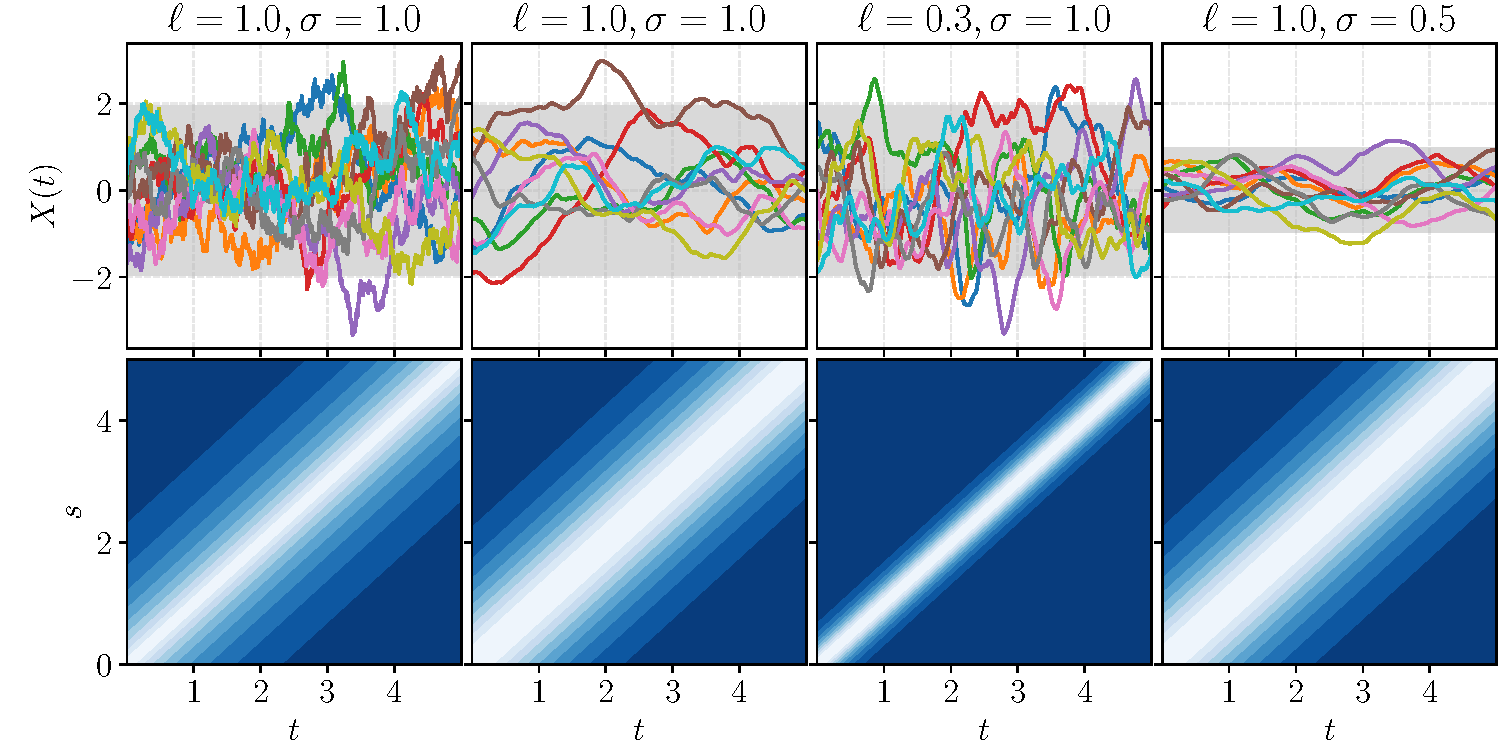
\includegraphics[width=.99\linewidth]{figs/sample-cov-matern}
		\caption{Samples (top) and covariance matrices (bottom) from Mat\'{e}rn GPs with $\nu=1 \, / \, 2$ (first column) and $\nu=3 / \, 2$ (other three columns).}
		\label{fig:matern}
	\end{figure}
	%
	The Mat\'{e}rn GP family has two distinctive parameters, that are, the length scale $\ell$ and magnitude (scale) $\sigma$. These two parameters, in a loose sense, control the ``correlation/variability/volatility'' of the GP in the horizontal and vertical directions. This is illustrated in Figure~\ref{fig:matern}.
\end{example}

Regarding the Mat\'{e}rn GPs, it is of interests to ask if we can let their parameters $\ell$ and $\sigma$ be functions of time. This is crucial in real-world modelling, because the underlying processes for many models are non-stationary, for example, in geostatistics~\citep{Higdon1999} and fluid mechanics~\citep{Monin1971}. The answer to the question is false, since the Mat\'{e}rn covariance function is in general not positive definite if we replace the parameters by any arbitrary function (e.g., $t \mapsto \ell(t)$). To solve this problem, \citet{Paciorek2004} craft a generalisation of the Mat\'{e}rn covariance function so that one can transform any stationary covariance function into a non-stationary one. \citet{Zhao2020SSDGP} show another way to construct non-stationary GPs from stochastic differential equations without explicitly using non-stationary covariance functions (see also Section~\ref{sec:sde-gp}).

\begin{example}[Radial basis GP]
	Since the Normal PDF is positive definite, we can borrow it as the covariance function of a GP too:
	%
	\begin{equation}
		C(t, s; \ell, \sigma) = \sigma^2 \exp\biggl(-\frac{1}{2} \, \Bigl(\frac{t - s}{\ell}\Bigr)^2\biggr),
		\label{equ:cov-rbf}
	\end{equation}
	%
	where parameters $\ell$ and $\sigma$ are similar to that of the Mat\'{e}rn family. Note that this covariance function is infinitely smooth in $t$ and $s$. This implies that the GP using this covariance function is infinitely smooth as well. 
	%
	\begin{figure}[t!]
		\centering
		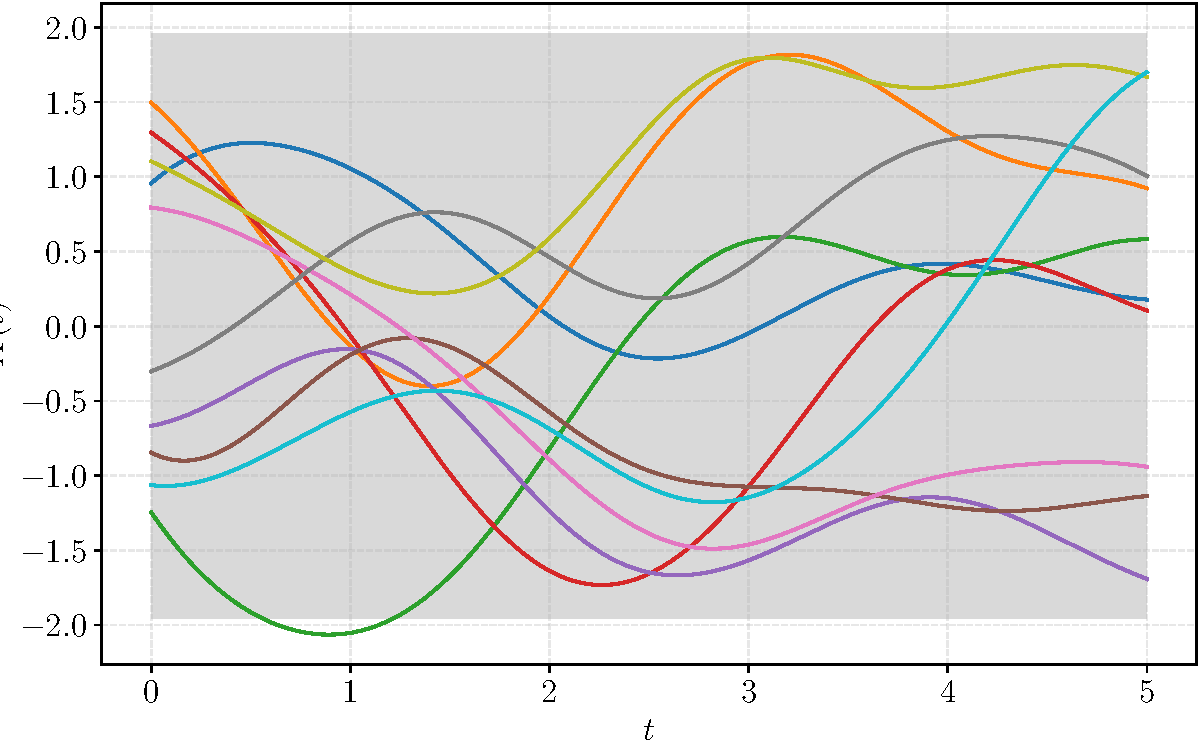
\includegraphics[width=.7\linewidth]{figs/sample-rbf}
		\caption{Samples from an RBF GP with $\ell=1$ and $\sigma=1$.}
		\label{fig:rbf}
	\end{figure}
	%
	Such smoothness makes the RBF GPs not often used in real applications.
	
	In the literature, this type of covariance function is often referred as ``squared exponential'', but I personally do not concur with this name, because it is really not by taking the square of the exponential covariance function. 
\end{example}

Many physicists argue against using the RBF covariance function in physical applications~\citep[see, e.g.,][]{Stein1999}, as the RBF GP is unrealistically too smooth. For example, we should not use the RBF GP to model the diffusion dynamics of particle/molecular in microscopic scale, because motion of particles/molecular is inherently not smooth. On the other hand, the fractional Brownian motion or the Mat\'{e}rn GPs may be used in this case, thanks to their capability of tuning the path regularity.

The RBF GP may also give numerical problems in the covariance matrix. The condition number of the RBF covariance matrix scales badly in the number of data points $T$.

\begin{example}[Sinusoidal GP]
	\label{example:sin-gp}
	Analogously to the example in Introduction, we can define a sinusoidal GP by
	%
	\begin{equation}
		X(t) = a \sin(t) + b \cos(t),
		\label{equ:equ:gp-cos}
	\end{equation}
	%
	where $a, b \sim \mathrm{N}(0, 1)$ are independent. The mean and covariance functions of this GP are
	%
	\begin{equation*}
		\begin{split}
			m(t) &= 0, \\
			C(t, s) &= \cos(s - t).
		\end{split}
	\end{equation*}
	%
	By the definition of this GP, we expect that the samples of it are sinusoidals with random amplitudes and phases. This is illustrated in Figure~\ref{fig:cos-gp}.
	%
	\begin{figure}[t!]
		\centering
		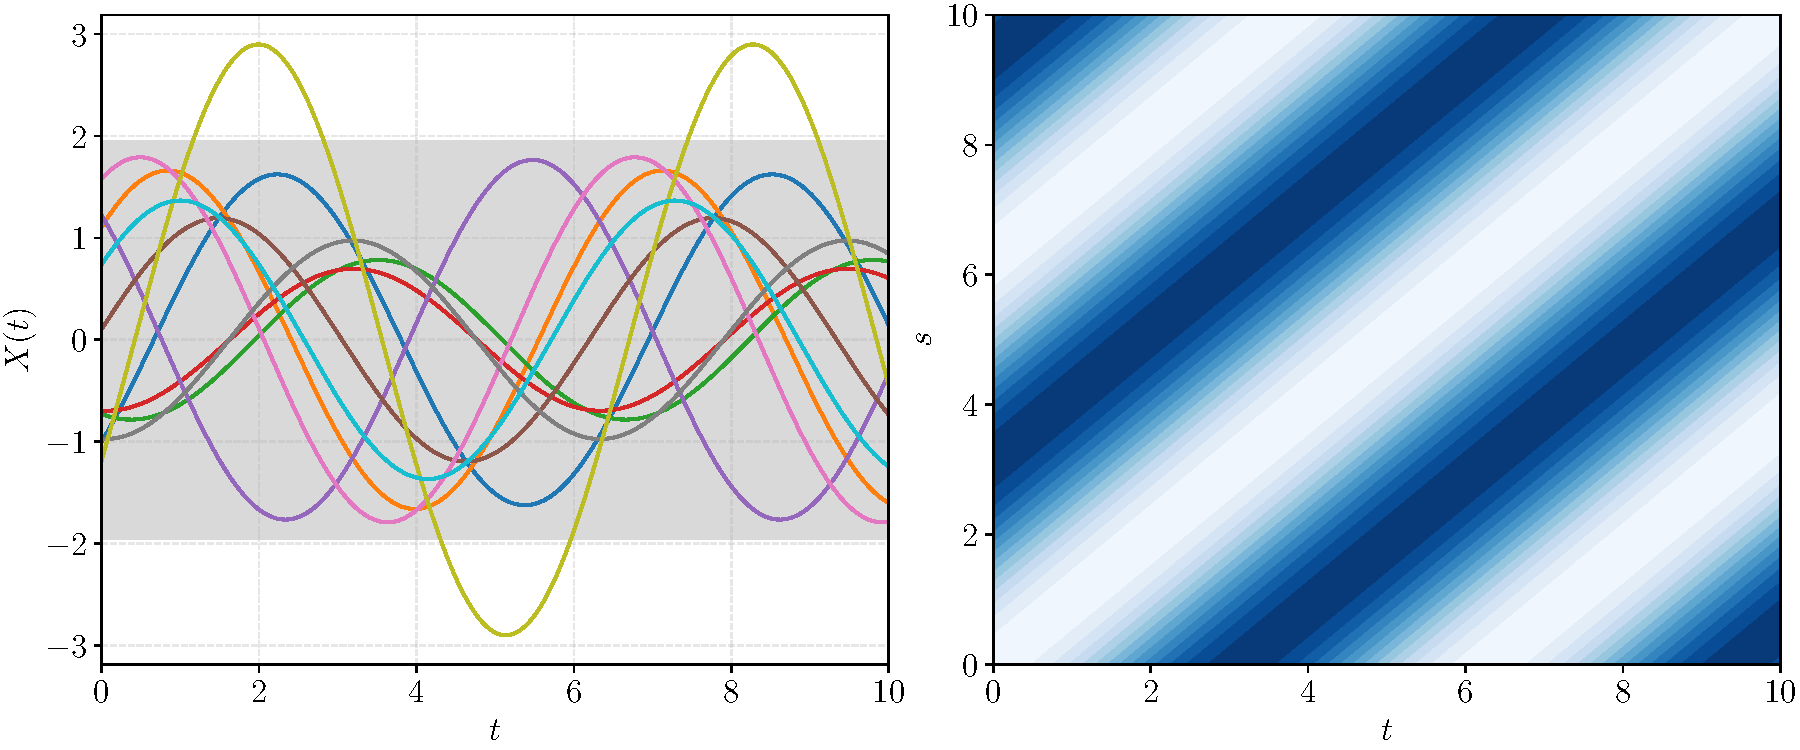
\includegraphics[width=.9\linewidth]{figs/sample-cov-cos}
		\caption{Samples (left) and covariance matrix (right) from a sinusoidal GP.}
		\label{fig:cos-gp}
	\end{figure}
	%
\end{example}

The examples above illustrate samples of GPs, yet, we have not learnt how to draw the GP samples. Drawing GP samples is trivial if we know the explicit construction of the GP, for example, in Equations~\eqref{equ:example-gp-linear-cov} and~\eqref{equ:equ:gp-cos}. However, in practice we do not know the explicit construction of GP, but only a pair of mean and covariance functions of it. In the following section, we show a number of approaches to  draw samples from a GP when its mean and covariance functions are given.

\section{Sampling from GP}
\label{sec:gp-sampling}
Suppose that we are given a GP
%
\begin{equation*}
	X(t) \sim \GP\bigl( m(t), C(t, t') \bigr)
\end{equation*}
%
with mean function $m$ and covariance function $C$. We would like to draw samples of $X$ evaluated at times $t_1, t_2, \ldots, t_T$. By the definition of GP, this is the same as with drawing samples from a vector of joint Normal random variables $X_{1:T} \coloneqq \begin{bmatrix} X(t_1) & X(t_2) & \cdots & X(t_T) \end{bmatrix} \in \R^T$ which follows a multivariate Normal PDF $\mathrm{N}(x_{1:T} \cond m_{1:T}, C_{1:T})$ (if such PDF exits). Of course in Python, you can simply call \texttt{numpy.random.multivariate\_normal}, but how would you actually implement this function? 

\subsection{Cholesky decomposition}
\label{sec:chol}
Let $\xi_{1:T}\coloneqq \begin{bmatrix}	\xi_1 & \xi_2 & \cdots & \xi_T \end{bmatrix} \in \R^T$ be a collection of $T$ independent identically distributed standard Normal random variables (i.e., $\mathrm{N}(0, 1)$), and suppose that we know how to draw samples from them. Then we can leverage $\xi_{1:T}$ to draw $X_{1:T}$ by the Cholesky decomposition $\sqrt{C_{1:T}}$ of the covariance matrix $C_{1:T}$. More precisely, the distribution of $X_{1:T}$ is the same as with 
%
\begin{equation}
	m_{1:T} + \sqrt{C_{1:T}} \, \xi_{1:T},
	\label{equ:chol}
\end{equation}
%
where $\sqrt{C_{1:T}}$ is the lower triangular matrix defined via $\sqrt{C_{1:T}} \, \sqrt{C_{1:T}}^\trans = C_{1:T}$ not the elementwise square root of $C_{1:T}$. This is true because any linear transformation of Normal random variables are Normal too, and the mean and covariance of the random variable $m_{1:T} + \sqrt{C_{1:T}} \, \xi_{1:T}$ match $m_{1:T}$ and $C_{1:T}$, respectively. This algorithm is summarised as follows.

\begin{algorithm}
	\SetAlgoLined
	\KwInput{Times $t_1, t_2, \ldots, t_T$, mean function $t \mapsto m(t)$, and covariance function $t,s \mapsto C(t,s)$}
	Compute $m_{1:T}$ and $C_{1:T}$ at the times\;
	Compute Cholesky decomposition $\sqrt{C_{1:T}}$\;
	Draw $\xi_{1:T}$\;
	$X_{1:T} = m_{1:T} + \sqrt{C_{1:T}} \, \xi_{1:T}$\;
	\KwRet{$X_{1:T}$}
	\caption{Draw a GP sample using Cholesky decomposition}
	\label{alg:chol}
\end{algorithm}

It is important to point out that we can understand this algorithm in terms of orthonormalisation (e.g., Gram--Schmidt process). To see this, let us first recall a basic result in linear algebra. Suppose that $\phi_1, \phi_2, \ldots, \phi_T$ are linearly independent basis functions, and define an inner product $\innerp{\cdot, \cdot}$. Then we can transform these linearly independent basis functions into a system of orthonormal basis by the Gram matrix of $\phi$'s. Formally, the Gram matrix is 
%
\begin{equation*}
	G \coloneqq 
	\begin{bmatrix}
		\innerp{\phi_1, \phi_1} & \innerp{\phi_1, \phi_2} & \cdots & \innerp{\phi_1, \phi_T} \\
		\innerp{\phi_2, \phi_1} & \innerp{\phi_2, \phi_2} & \cdots & \innerp{\phi_2, \phi_T} \\
		\vdots & \vdots & \ddots & \vdots \\
		\innerp{\phi_T, \phi_1} & \innerp{\phi_T, \phi_2} & \cdots & \innerp{\phi_T, \phi_T}
	\end{bmatrix},
\end{equation*}
%
and the new functions $\psi_1, \psi_2, \ldots, \psi_T$ defined via
%
\begin{equation*}
	\psi_i \coloneqq \sum_{j=1}^T (\sqrt{G}^{-1})_{ij} \, \phi_j, \quad i=1,2,\ldots, T,
\end{equation*}
%
are orthonormal in terms of $\innerp{\cdot, \cdot}$. Please prove this result as an exercise. If you prefer to use the vector notation, the result writes
%
\begin{equation*}
	\begin{bmatrix}
		\psi_1 \\
		\psi_2 \\
		\vdots \\
		\psi_T
	\end{bmatrix}
	 = 
	 \sqrt{G}^{-1}
	\begin{bmatrix}
		\phi_1 \\
		\phi_2 \\
		\vdots \\
		\phi_T
	\end{bmatrix}.
\end{equation*}
%

To apply this result in our case, let us define the functions by $\phi_i(x) \coloneqq x_i - m_i$ which selects the $i$-th element of its argument $x\in\R^T$ then subtracts the corresponding mean component. It is clear that $\phi_1, \phi_2, \ldots, \phi_T$ are linearly independent. For any two (Normal) random variables $Y$ and $Z$, let us define their inner product by $\innerp{Y, Z} \coloneqq \expec{Y \, Z}$, then $\innerp{\phi_i(X_{1:T}), \phi_j(X_{1:T})} = \expec{(X_i - m_i) \, (X_j - m_j)} = C(t_i, t_j)$. Therefore, the Gram matrix here is indeed our covariance matrix. Let $\xi_i \coloneqq \psi_i(X_{1:T})$. Evidently, $\psi_1, \psi_2, \ldots, \psi_T$ are orthonormal in the inner product from the orthonormalisation process. Finally, we have
%
\begin{equation*}
	X_{1:T} = 
	\begin{bmatrix}
		\phi_1 \\
		\phi_2 \\
		\vdots \\
		\phi_T
	\end{bmatrix} + m_{1:T} =
	\sqrt{C_{1:T}}
	\begin{bmatrix}
		\psi_1 \\
		\psi_2 \\
		\vdots \\
		\psi_T
	\end{bmatrix} + m_{1:T}
\end{equation*}
%
which equals to Equation~\eqref{equ:chol}. Essentially, we use the inverse of the Cholesky decomposition $\sqrt{C_{1:T}}^{-1}$ of the covariance matrix to whitten $X_{1:T}$. This is also equivalent to say that we use $\sqrt{C_{1:T}}$ to transform the whittened $\xi_{1:T}$ back to $X_{1:T}$. 

It is also worth noting a numerical issue of the Cholesky approach. This approach is sensitive to the condition number of the covariance matrix. For instance, when the times $t_1, t_2, \ldots, t_T$ are densely located, the covariance matrix $C_{1:T}$ can be numerically ill-conditioned.

\subsection{Spectral decomposition}
\label{equ:eigendecomposition}
We can generalise the Cholesky decomposition algorithm by eigendecompositions of the covariance matrix. Since $C_{1:T}$ is symmetric positive semi-definite, its eigenvalues are all real and non-negative hence, we can decomposite it by 
%
\begin{equation*}
	C_{1:T} = U \, V \, U^\trans, 
\end{equation*}
%
where columns in $U \in\R^{T\times T}$ are the (orthonormal) eigenvectors, and $V\in\R^{T\times T}$ is a diagonal matrix containing the corresponding eigenvalues. Then,
%
\begin{equation*}
	m_{1:T} + U \sqrt{V} \, \xi_{1:T}
\end{equation*}
%
has the same distribution as $X_{1:T}$. We can also equivalently write the equation above in another fashion if you prefer
%
\begin{equation*}
	m_{1:T} + \sum^T_{i=1} \sqrt{v_j} \, \xi_j \, u_j,
\end{equation*}
%
where $v_j \geq 0$ and $u_j \in\R^{T}$ are the $j$-th eigenvalue and eigenvector, respectively.

Compared to the Cholesky decomposition approach, this spectral decomposition allows $C_{1:T}$ to have zero eigenvalue(s).  

\subsection{Computational complexity}
The computational complexity of Algorithm~\ref{alg:chol} is $O(T^3)$, because the dominating procedure in the algorithm is computing the Cholesky decomposition $\sqrt{C_{1:T}}$ which is (nearly) cubic in $T$. The spectral decomposition approach has a similar cubic complexity too. This means that the sampling algorithms presented above are computationally invalid if the number of times $T$ is large, not to mention that it is hard to store a dense matrix $C_{1:T}$ of huge size $T\times T$ nevertheless. Therefore, in the following three sections, we show a few alternative sampling methods that suffer less from this computational problem.

\subsection{Approximate sampling with L\'{a}nczos interation}
\label{sec:lanczos}
Recall the spectral decomposition of $X_{1:T}$ formulated previously:
%
\begin{equation*}
	m_{1:T} + \sum^T_{i=1} \sqrt{v_j} \, \xi_j \, u_j.
\end{equation*}
%
If $T$ is large, we may approximate the decomposition by a truncation
%
\begin{equation*}
	\widehat{X}_S \coloneqq m_{1:T} + \sum^S_{i=1} \sqrt{v_j} \, \xi_j \, u_j
\end{equation*}
%
for some small number $S \ll T$, so that we do not need to compute all the eigenvalues and eigenvectors. But, how do we find/select the number $S$, and how to select the eigenvalues $\lbrace v_i \rbrace_{1=1}^S$ in order to have a good approximation? A heuristic solution is to sort all the eigenvalues $\lbrace v_i \rbrace_{1=1}^T$ then select the $S$ biggest ones. But to sort them, we need to compute all the eigenvalues which is the problem that we were trying to avoid. 

We could find the $S$-most useful eigenvalues (and eigenvectors) by using the L\'{a}nczos algorithm~\citep[see,][Ch. 10]{Golub2013}. This algorithm forms a tridiagonal matrix $\widehat{V} \in \R^{S \times S}$ and another orthonormal matrix $\widehat{U}\in\R^{T \times S}$ in the way that
%
\begin{equation*}
	\widehat{V} = \widehat{U}^\trans \, C_{1:T} \, \widehat{U}.
\end{equation*}
%
This algorithm is fast, since it can find the matrix $\widehat{U}$ and the non-zero elements of $\widehat{V}$ in one loop of size $m$. Furthermore, if $v$ and $u$ is a pair of eigenvalue and eigenvector of $\widehat{V}$, then $v$ and $\widehat{U} \, u$ are an pair of eigenvalue and eigenvector of $C_{1:T}$ (this holds when $S=T$). Therefore, we can use this algorithm to approximate the spectral decomposition of $C_{1:T}$ by a smaller decomposition problem of $\widehat{V}$. Since $\widehat{V}$ is tridiagonal, finding its eigenvalues and eigenvectors can be far cheaper than the original cubic complexity. For instance, \citet{Coakley2013} compute the eigenvalues in a subquadratic complexity. However, the downside of the L\'{a}czos approach is that it can be numerically unstable and is picky for $C_{1:T}$, the matrix of which should have extremal eigenvalues.

\begin{figure}[t!]
	\centering
	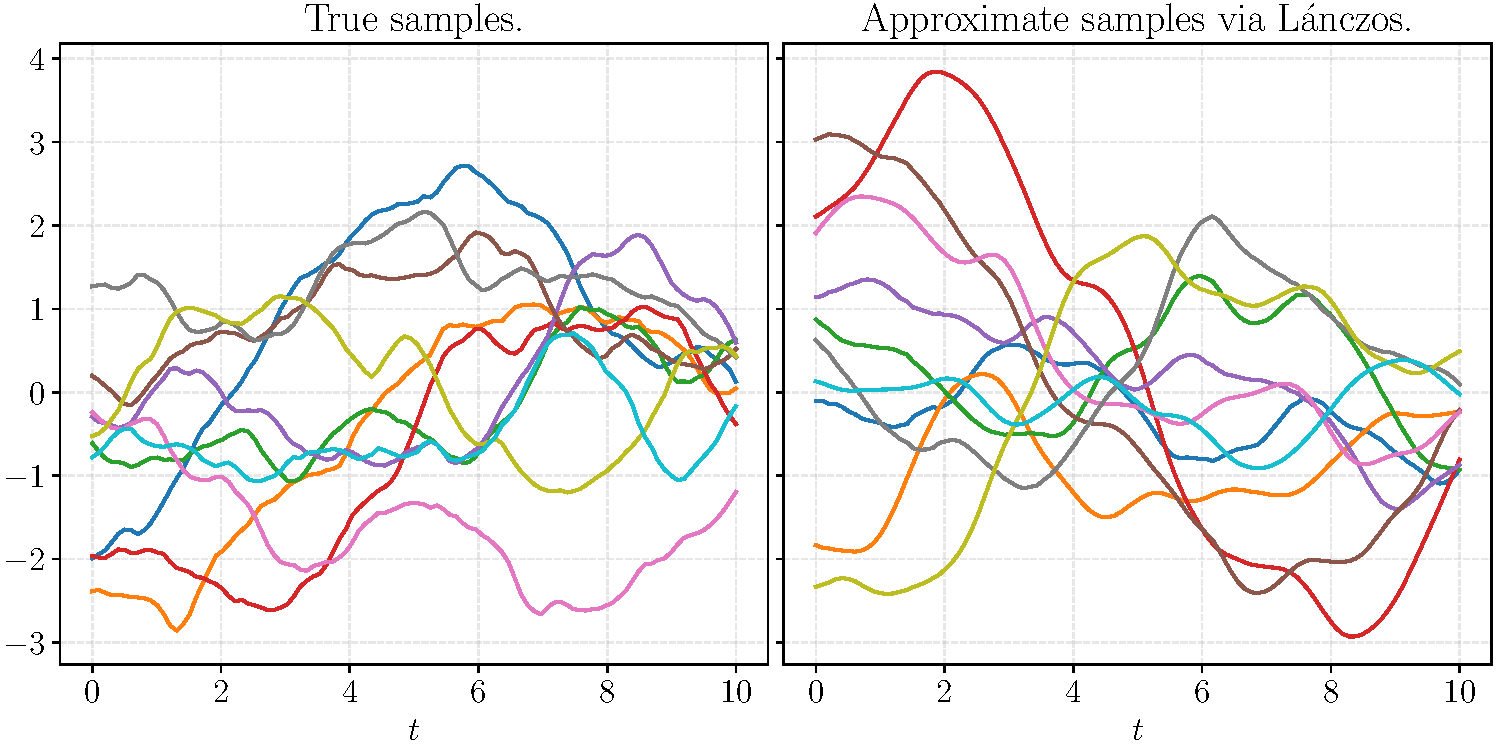
\includegraphics[width=.9\linewidth]{figs/lanczos-demo}
	\caption{Approximate samples by using L\'{a}nczos iteration for a Mat\'{e}rn $\nu=3 \, / \, 2$ GP. In this demonstration, we let $T = 100$ and $S=20$.}
	\label{fig:lanczos-gp}
\end{figure}

In Figure~\ref{fig:lanczos-gp}, we show an example of applying the L\'{a}nczos algorithm to make (approximate) samples from a Mat\'{e}rn GP. From this figure, we find that the samples produced by the L\'{a}nczos algorithm approximate the true samples to a reasonable extent. However, since we have discarded many eigenvalues, the path of the approximate sample appears smoother than that of the true sample.

For the sake of simplicity, we prefer not to detail more about the L\'{a}nczos algorithm, but we kindly refer the readers to, for example, the monograph by \citet{Golub2013} for more insights.

\subsection{Kosambi--Karhunen--Lo\`{e}ve expansion}
\label{sec:karhunen-loeve}
The crux of the mentioned computational problem is that we were thinking the stochastic process as a collection of random variables, because sampling from \emph{high-dimensional} vector space is challenging. To avoid this problem, we now need to rethink the stochastic process as a function-valued random variable. That is, instead of drawing sample of the process evaluated at finite times, we draw the sample path entirely as a function from an \emph{infinite-dimensional} space. We introduce the Kosambi--Karhunen--Lo\`{e}ve (KKL) expansion as follows.

Suppose that $X\colon \Omega \to L^2(D)$ is a square-integrable process (you can find the precise definition of ``square-integrable $L^2$'' in many probability theory textbooks) on some domain $D \subset [0, \infty)$, and that $\lbrace \varphi_1, \varphi_2, \ldots \rbrace$ is any set of orthonormal basis of $L^2(D)$, then we can expand the process in the way that
%
\begin{equation*}
	X(t) = m(t) + \sum_{i=1}^\infty \lambda_i \, \varphi_i(t),
\end{equation*}
%
for all $t\in D$, where the coefficient $\lambda_i$ is random and is given by
%
\begin{equation*}
	\lambda_i = \innerp{X - m, \varphi_i}_{L^2(D)}.
\end{equation*}
%
There are of course many orthonormal basis systems in the space. Since in our context we know the covariance function $C$ of the process, we can choose $\lbrace \lambda_1, \lambda_2, \ldots \rbrace$ and $\lbrace \varphi_1, \varphi_2, \ldots \rbrace$ from the eigenvalues and eigenfunctions of an integral operator $K$ defined by
%
\begin{equation*}
	(K f)(t) \coloneqq \int_D C(t, s) \, f(s) \diff s, \quad f \in L^2(D).
\end{equation*}
%
Now let $\lbrace v_i, \varphi_i \rbrace_{i=1}^{\cdots}$ be the eigenvalues and eigenfunctions of $K$, then the KKL expansion is such that
%
\begin{equation*}
	X(t) = m(t) + \sum_{i=1}^\infty \sqrt{v_i} \, \xi_i \, \varphi_i(t),
\end{equation*}
%
where $\expec{\xi_i} = 0$, $\varr{\xi_i} = 1$, and $\lbrace \xi_1, \xi_2, \ldots \rbrace$ are mutually uncorrelated (prove this as an exercise). If $X$ is a GP, $\lbrace \xi_1, \xi_2, \ldots \rbrace$ are then independent standard Normal random variables. The covariance function is also such that $C(t, s) = \sum_{i=1}^\infty v_i \, \varphi_i(t) \, \varphi_j(s)$ by Mercer's theorem.

The KKL expansion implies that we can approximate samples of $X$ by samples from independent Normal random variables which are easy to sample from. We summarise the algorithm in the following.

\begin{algorithm}
	\SetAlgoLined
	\KwInput{Mean function $t \mapsto m(t)$, and covariance function $t,s \mapsto C(t,s)$, expansion order $N$.}
	Derive the eigenvalues and eigenfunctions of the oprator $K$, then order them and select the first $N$ ones $\lbrace v_i, \varphi_i \rbrace_{i=1}^{N}$\;
	Draw independent Normal random variables $\lbrace \xi_1, \xi_2, \ldots, \xi_N\rbrace$\;
	\Func{$X(t)$:}{\KwRet{} $m(t) + \sum_{i=1}^N \sqrt{v_i} \, \xi_i \, \varphi_i(t)$}
	\KwRet{$X$}
	\caption{Approximate GP using KKL expansion}
	\label{alg:kkt}
\end{algorithm}

The downside of the KKL approach is that we need to derive the eigenvalues and eigenfunctions of the integral operator from the given covariance function. This is analytically doable only for a few isolated cases, for example, the expansion of Brownian motion as shown in the following example. Otherwise, one has to approximate them numerically.

\begin{example}
	\label{example:kkt-bm}
	Let $C(t,s) = \min(t,s)$, and $D = [0, 1]$, then the eigenfunctions and eigenvalues of the operator $K$ are given by
	%
	\begin{equation*}
		\begin{split}
			\varphi_i(t) &= \sqrt{2} \sin\biggl( \Bigl(i - \frac{1}{2} \Bigr) \, \pi \, t \biggr), \\
			v_i &= \frac{1}{\bigl(i - \frac{1}{2} \bigr)^2 \, \pi^2},
		\end{split}
	\end{equation*}
	%
	for $i=1,2,\ldots$ and $t\in[0, 1]$. See, for example, \citet[][pp. 205]{Lord2014} for the derivation. We illustrate an example of this expansion in Figure~\ref{fig:kkt-bw} with increasing order of truncation $N$.
\end{example}

\begin{figure}[t!]
	\centering
	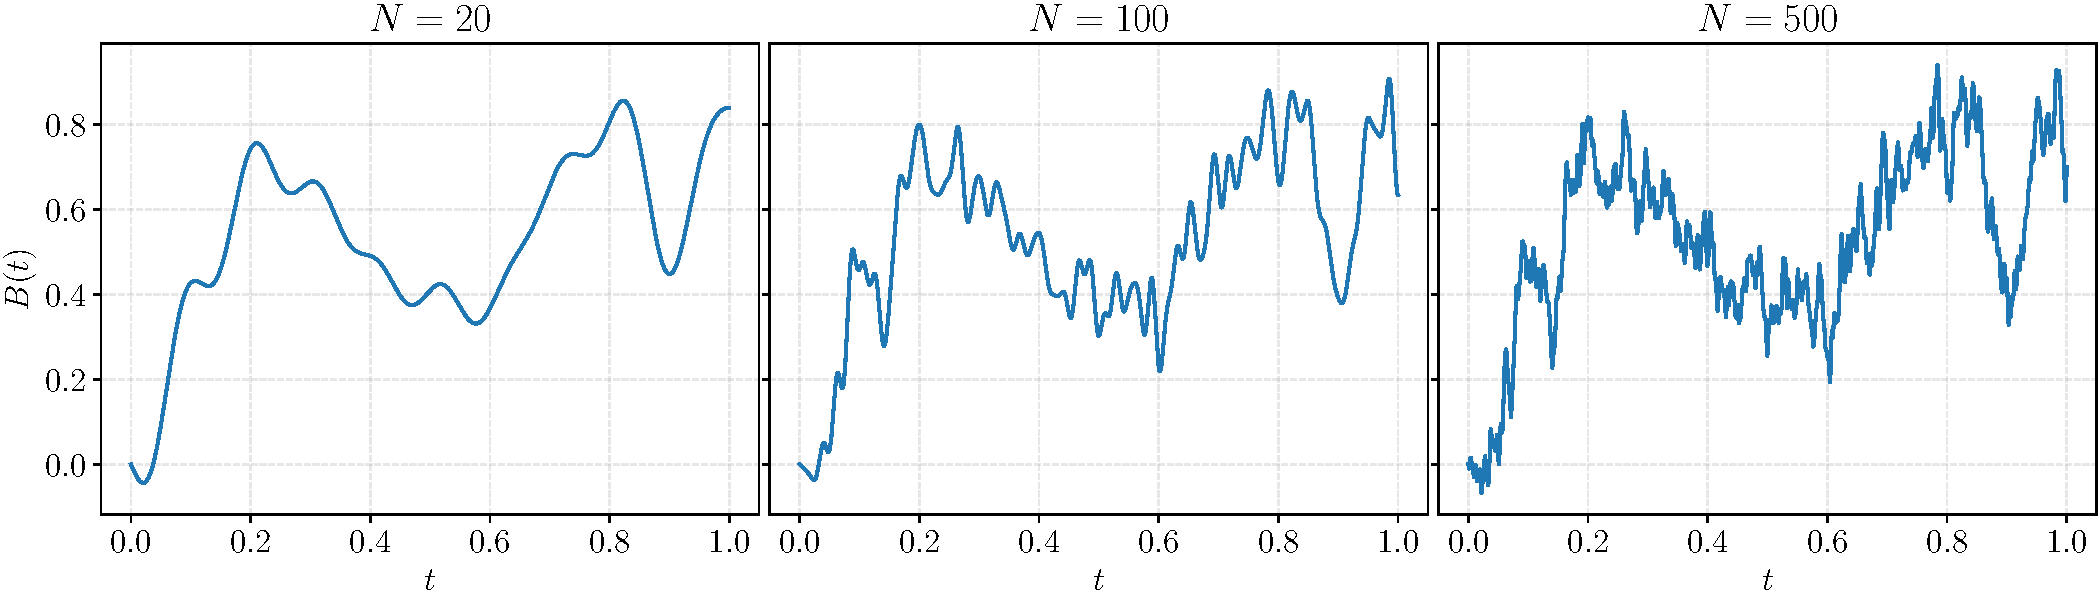
\includegraphics[width=.98\linewidth]{figs/kkl-bw}
	\caption{KKL expansion of a Brownian motion sample with increasing truncation order $N$. The approximate sample path is getting closer to the true one as $N$ increases.}
	\label{fig:kkt-bw}
\end{figure}

\begin{remark}
	Example~\ref{example:kkt-bm} gives an KKL expansion of Brownian motion
	%
	\begin{equation*}
		B(t) = \sum^\infty_{i=1} \frac{\sqrt{2}}{\bigl(i - \frac{1}{2} \bigr) \, \pi} \sin\biggl( \Bigl(i - \frac{1}{2} \Bigr) \, \pi \, t \biggr).
	\end{equation*}
	%
	Now take a derivative of any summand above, we get
	%
	\begin{equation*}
		\sqrt{2} \cos\biggl( \Bigl(i - \frac{1}{2} \Bigr) \, \pi \, t \biggr).
	\end{equation*}
	%
	Here you should note is that for the cosine component in the equation above, its amplitude is a constant $\sqrt{2}$ which is independent of the frequency index $i$. This says that the spectral density of the ``derivative'' process is white. Indeed, one can define the white noise process as the formal derivative of Brownian motion.
\end{remark}

\subsection{Circulant embedding for stationary GPs}
\label{sec:circulant-embedding}
The truncated spectral decomposition and KKL expansion methods are efficient indeed, however, we should note that these methods are approximate. If one wants to make exact GP samples, and the covariance function being symmetric positive definite is the only information that we know, then we cannot really do better than the Cholesky decomposition method. In order to develop a more efficient sampling method, either we should know the explicit construction of the GP (e.g., Examples~\ref{example:affine-gp} and~\ref{example:sin-gp}), or we should know some additional information/structure of the covariance function/matrix at hand. To elucidate this argument, let us consider two extreme examples as follows. 

Suppose that we have a GP with covariance function $C(t,s) = 1$. In addition to knowing that the covariance matrix is positive semi-definite, we also know that the covariance matrix is an all-one matrix. Therefore, to make a sample from this GP, we simply draw from a Normal random variable $X_0$ then let $X(t) = X_0$ for any query $t$. As another example, if the covariance matrix is diagonal, then the sample of the underlying GP is a collection of independent Normal random variables which are trivial to sampling. In these two examples, we can draw GP samples in one-shot because we leverage the structures of their covariance matrices. On the other hand, covariance functions in reality are much more complicated than these two extreme examples.

In what follows, we present an exact GP sampling method that applies to a wide family of GPs that are stationary~\citep{Wood1994, Chan1997}. The stationary GPs cover a plenty of useful covariance functions, for instance, Mat\'{e}rn and radial basis functions which are commonly used by the GP practitioners. The essence of this method is the fact that the covariance matrix of any stationary GP has a circulant extension. Therefore, we can leverage this circulant matrix structure to form a decomposition of the covariance matrix by discrete Fourier transform which can be computed lighting fast. To explain this method, let us start by the definition of stationary GPs.

\begin{definition}[Stationary process]
	\label{def:stationary-gp}
	A stochastic process $X\colon [0, \infty) \to \R$ is said to be stationary if for all $T\geq 1$ and reals $t_1 < t_2 < \ldots < t_T \in [0, \infty)$, the distribution of $\lbrace X(t_1), X(t_2), \ldots, X(t_T) \rbrace$ is the same with the distribution of $\lbrace X(t_1 + \tau), X(t_2 + \tau), \ldots, X(t_T + \tau) \rbrace$ for all translation $\tau$.
\end{definition}

Definition~\ref{def:stationary-gp} means that the finite-dimensional distribution of the process is invariant under translation. Imagine that you select a time window of fixed length, the distribution of the stationary process in the time window must not change if you shift the time window, and this result must hold for arbitrary window length and position.

Now consider zero-mean GPs. We say that the GP is stationary if its covariance function $C(t,s) = C(t+\tau, s+\tau)$ for all $t,s,\tau$, viz., the covariance function depends on the time difference $t-s$ only. The covariance matrices of stationary GPs are closely related to symmetric Toeplitz matrices.

% Bochner, Winer--Khinchin

\begin{definition}[Symmetric Toeplitz matrix]
	We say that a matrix $A\in\R^{T \times T}$ is symmetric Toeplitz of first column $\begin{bmatrix} a_0 & a_1 & \cdots & a_{T-1} \end{bmatrix} \in\R^T$, if the element of the matrix satisfies $A_{ij} = a_{\abs{i-j}}$ for all indices $1\leq i,j\leq T$. That is,
	%
	\begin{equation*}
		A = 
		\begin{bmatrix}
			a_0 & a_1 & \cdots & a_{T-2} & a_{T-1} \\
			a_1 & a_0 & a_1 & \ddots & a_{T-2} \\
			\vdots & \ddots & \ddots & \ddots & \vdots \\
			a_{T-2} & \ddots & a_1 & a_0 & a_1 \\
			a_{T-1} & a_{T-2} & \cdots & a_1 & a_0
		\end{bmatrix}.
	\end{equation*}
	%
\end{definition}

\begin{proposition}
	\label{prop:cov-fisrt-col}
	Suppose that the times $t_1, t_2, \ldots, t_T$ are evenly placed, that is, $t_2 - t_1 = t_3 - t_2 = \ldots = t_T - t_{T-1}$. Then the covariance matrix $C_{1:T}\in\R^{T\times T}$ of any stationary GP at these times is symmetric Toeplitz of first column $\begin{bmatrix} C(t_1, t_1) & C(t_2, t_1) & \cdots & C(t_{T}, t_1) \end{bmatrix} \in\R^T$.
\end{proposition}
\begin{proof}
	This is concluded by definition.
\end{proof}

The proposition above says that the covariance matrix of stationary GP is completely determined by a vector which is its first column. This means that on a computer we do not need to store the entire dense matrix but its first column vector only; For any algebra that operates on the covariance matrix, we may do algebras on its first column. 

Next, we show that every symmetric Toeplitz matrix has a (minimal) circulant extension, the result of which we use to make GP samples. 

\begin{definition}[Circulant matrix]
	A matrix $A\in\R^{T\times T}$ is called circulant of first column $\begin{bmatrix} a_0 & a_1 & \cdots & a_{T-1} \end{bmatrix} \in\R^T$, if elements of the matrix are such that $A_{ij} = a_{i-j}$ for all $1\leq j\leq i$ and $A_{ij}=a_{i-j+T}$ for all $i+1\leq j\leq T$. That is, every column of the matrix is a one-step cyclic shift of its preceding column:
	%
	\begin{equation*}
		A = 
		\begin{bmatrix}
			a_0 & a_{T-1} & \cdots & a_2 & a_1 \\
			a_1 & a_0 & \ddots & \vdots & a_2 \\
			\vdots & a_1 & \ddots & \vdots & \vdots \\
			a_{T-2} & \vdots & \ddots & a_0 & a_{T-1} \\
			a_{T-1} & a_{T-2} & \cdots & a_1 & a_0
		\end{bmatrix}
	\end{equation*}
	%
	Circulant matrix is symmetric if its first column satisfies $a_{T-i} = a_i$ for $i=1,2,\ldots,T-1$.
\end{definition}

It turns out that every symmetric Toeplitz matrix, hence, every stationary GP covariance matrix (with evenly placed times) has a symmetric circulant extension.

\begin{proposition}
	\label{prop:first-col-ext}
	Every symmetric Toeplitz matrix $A\in\R^{T\times T}$ of first column $\begin{bmatrix} a_0, a_1, \ldots, a_{T-1} \end{bmatrix} \in \R^T$ has an extension matrix $\overline{A}$ that is symmetric circulant of first column $\begin{bmatrix} a_0, a_1, \ldots, a_{T-1}, a_{T-2}, \ldots, a_{1}\end{bmatrix} \in \R^{2 \, T - 2}$. The extension means an embedding that
	%
	\begin{equation*}
		\overline{A} = 
		\begin{bmatrix}
			A & B \\
			B^\trans & E
		\end{bmatrix}
	\end{equation*}
	%
	for some matrices $B$ and $E$. Furthermore, this $\overline{A}$ is the smallest circulant matrix that can embed $A$.
\end{proposition}

\begin{example}
	Consider a covariance function $C(t,s) = \exp(-\abs{t - s})$ and times $t_1=1$, $t_2 = 2$, and $t_3 = 3$. The covariance matrix $C_{1:3}$ reads
	%
	\begin{equation*}
		C_{1:3} = 
		\begin{bmatrix}
			1 & \expp^{-1} & \expp^{-2} \\
			\expp^{-1} & 1 & \expp^{-1} \\
			\expp^{-2} & \expp^{-1} & 1
		\end{bmatrix}
	\end{equation*}
	%
	which is a symmetric Toeplitz matrix of first column $\begin{bmatrix} 1 & \expp^{-1}	& \expp^{-2}\end{bmatrix}$. Its minimal circulant extension is
	%
	\begin{equation*}
		\begin{bmatrix}
			1 & \expp^{-1} & \expp^{-2} & \expp^{-1}\\
			\expp^{-1} & 1 & \expp^{-1} & \expp^{-2}\\
			\expp^{-2} & \expp^{-1} & 1 & \expp^{-1}\\
			\expp^{-1} & \expp^{-2} & \expp^{-1} & 1
		\end{bmatrix}
	\end{equation*} 
	%
	of first column $\begin{bmatrix} 1 & \expp^{-1}	& \expp^{-2} & \expp^{-1}\end{bmatrix}$.
\end{example}

\begin{remark}
	Although the minimal circulant extension of any symmetric Toeplitz is symmetric, the extension might not be non-negative definite. This specifically depends on the covariance function at hand.
\end{remark}

Suppose that the minimal circulant $\overline{C}_{1:n} \in \R^{n \times n}$ of the covariance matrix $C_{1:T}$ is positive semi-definite, where $n=2\,T-2$. We can make samples according to $\overline{C}_{1:n}$ then slice the first $T$ components of the samples to get the samples from that of $C_{1:T}$. This seems to be a fuss, since the size of the extension $\overline{C}_{1:n}$ is bigger than $C_{1:T}$. However, thanks to a remarkable Fourier representation of circulant matrix, it is indeed worth sampling from $\overline{C}_{1:n}$.

\begin{proposition}
	Any circulant matrix $A\in \R^{n\times n}$ of first column $a_{0:n-1} \coloneqq \begin{bmatrix} a_0 & a_1 & \cdots & a_{n-1} \end{bmatrix} \in \R^n$ has a Fourier representation
	%
	\begin{equation*}
		A = F \, D \, F^\star,
	\end{equation*}
	%
	where $F \in \mathbb{C}^{n \times n}$ is a Fourier matrix with element 
	%
	\begin{equation*}
		F_{ij} \coloneqq \frac{1}{\sqrt{n}} \, \bigl(\expp^{-2 \, \pi \, \imag \, / \, n} \bigr)^{(i - 1) \, (j - 1)},
	\end{equation*}
	%
	and $D$ is a diagonal matrix with diagonal $\sqrt{n} \, F^\star \, a_{0:n-1}$. The star superscript means conjugate transpose.
\end{proposition}

\begin{remark}
	The Fourier matrix is such that $\sqrt{n} \, F \, a$ and $\frac{1}{\sqrt{n}} \, F^\star \, a$ represent the discrete Fourier transform (DFT) and the inverse DFT for any vector $a$, respectively.
\end{remark}

The Fourier representation in the proposition above suggests that to sample according to a circulant matrix we can combine the inverse DFT of the first column, and samples from complex Normal random variables. This is detailed in the following proposition.

\begin{proposition}
	Let $\xi_{1:n} \in \mathbb{C}^{n}$ be a vector of standard complex Normal random variables, and suppose that the minimal circulant extension $\overline{C}_{1:n}$ of the covariance matrix $C_{1:T}$ is positive semi-definite. Let $X^1_{1:T}$ and $X^2_{1:T}$ be the first $T$ components of 
	%
	\begin{equation*}
		\mathrm{Re} \bigl(F \, \sqrt{D} \, \xi_{1:n} \bigr) \quad \text{and} \quad \mathrm{Im} \bigl(F \, \sqrt{D} \, \xi_{1:n} \bigr),
	\end{equation*}
	%
	respectively, where the diagonal of $D$ is $\sqrt{n} \, F^\star \, \overline{c}_{1:n}$, and $\overline{c}_{1:n}$ is the first column of $\overline{C}_{1:n}$. Then, $X^1_{1:T}$ and $X^2_{1:T}$ are independent identically distributed, and the distribution is $\mathrm{N}(0, C_{1:T})$.
\end{proposition}

To compute the DFT and inverse DFT in practice, we use the fast Fourier transform (FFT) algorithm. The computational complexity of FFT is $O(n\log n)$ which is significantly smaller than $O(T^3)$ when $T$ is large. We summarise the sampling method in the following algorithm, and exemplify a result from the algorithm in Figure~\ref{fig:circulant-sample}.

\begin{algorithm}
	\SetAlgoLined
	\KwInput{Evenly placed times $t_1, t_2, \ldots, t_T$, mean function $t \mapsto m(t)$, and covariance function $t,s \mapsto C(t,s)$}
	$n = 2 \, T - 2$\;
	Compute $m_{1:T}$ at the times\;
	Compute the first column $c_{0:T-1}$ as per Proposition~\ref{prop:cov-fisrt-col}\;
	Compute the circulant first column extension $\overline{c}_{1:n} \in \R^{n}$ of $c_{0:T-1}$ as per Proposition~\ref{prop:first-col-ext}\;
	$d_{1:n} = n * \texttt{ifft}(\overline{c}_{1:n})$\;
	Draw independent $\alpha, \beta\sim\mathrm{N}(0,I_{n})$ and let $\xi_{1:n} = \alpha + \beta \, \imag$\;
	Elementwise vector multiplication $z_{1:n}=\sqrt{d_{1:n}} \, \xi_{1:n}$\;
	Let $g_{1:T}$ be the first $T$ components of $\texttt{fft}(z_{1:n}) \, / \, \sqrt{n}$\;
	\KwRet{Two indepedent samples $m_{1:T} + \texttt{real}(g_{1:T})$ and $m_{1:T} + \texttt{imag}(g_{1:T})$}
	\caption{Sampling from stationary GP by minimal circulant embedding}
	\label{algo:circulant-embedding}
\end{algorithm}

\begin{figure}[t!]
	\centering
	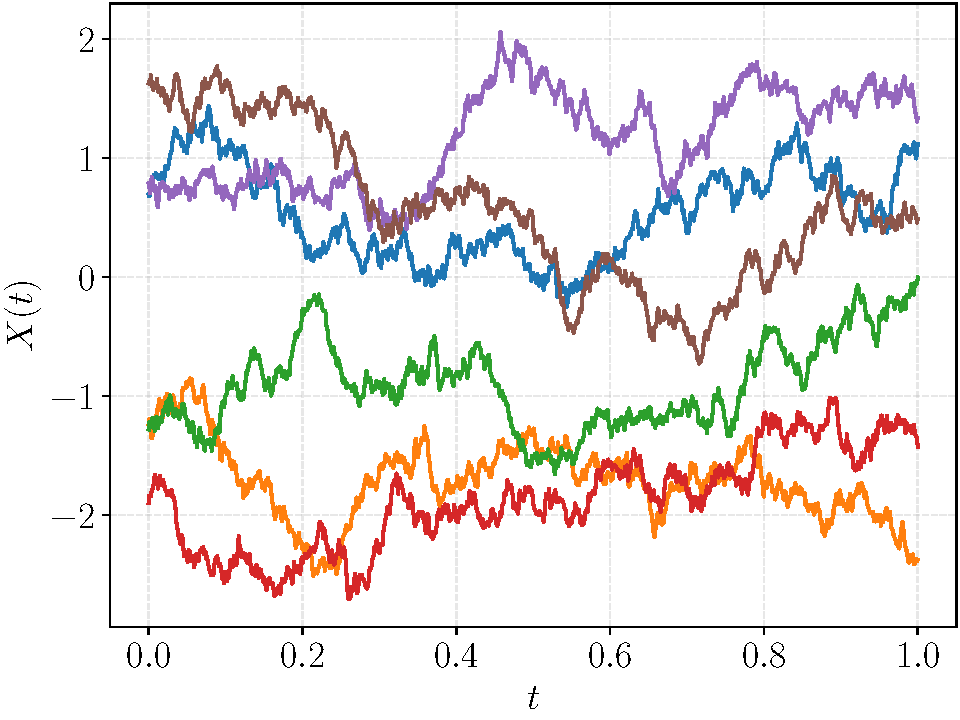
\includegraphics[width=.6\linewidth]{figs/circulant-gp-sample}
	\caption{Samples from a GP with exponential covariance function ($\ell=1$, $\sigma=1$) by using Algorithm~\ref{algo:circulant-embedding}. Try run the code while setting $T$ to be mega big, compare with the Cholesky approach, and have fun.}
	\label{fig:circulant-sample}
\end{figure}

\begin{exercise}
	What if the times are not evenly placed? If this is true, the covariance matrix is not symmetric Toeplitz. How to remedy this problem?
\end{exercise}

\section{Regression}
\label{sec:regression}
In this section we show how to solve a GP regression problem from the model of the form
%
\begin{equation}
	\begin{split}
		X(t) &\sim \GP\bigl( m(t), C(t, t') \bigr), \\
		Y_k &= a \, X(t_k) + b + \xi_k,
		\label{equ:gp-regression-model}
	\end{split}
\end{equation}
%
where the random variable $Y_k \in \R$ represents the measurement of the GP $X$ at time $t_k$ through any affine transformation defined via $a\neq 0$, $b$, and measurement noise $\xi_k \sim \mathrm{N}(0, \Xi)$. Now suppose that we have a set of measurements/data $y_{1:T} \coloneqq \lbrace y_1, y_2, \ldots, y_T\rbrace$ from $Y_{1:T}$ at times $t_1, t_2,\ldots, t_T$, the goal is to solve the posterior distribution of $X$ conditionally on these measurements. More specifically, we would like to solve the posterior density
%
\begin{equation*}
	p(x_{1:T} \cond y_{1:T}) = \mathrm{N}(x_{1:T} \cond \alpha_{1:T}, \beta_{1:T})
\end{equation*}
%
of $X_{1:T}$ given $Y_{1:T} = y_{1:T}$. Since the measurement random variables and the GP are jointly Normal distributed, the posterior distribution is Normal as well, with mean $\alpha_{1:T} \coloneqq \expec{X_{1:T} \cond y_{1:T}}$ and covariance $\beta_{1:T} \coloneqq \cov{X_{1:T} \cond y_{1:T}}$. To obtain the posterior mean and covariance, we recall the Gaussian identity that we learnt from the previous lecture on Bayesian linear regression.

\begin{proposition}[Gaussian identity]
	\label{prop:gaussian-identity}
	Let $X_{1:T}\in\R^{T}$ and $Y_{1:T} \in \R^T$ be jointly Normal such that
	%
	\begin{equation*}
		\begin{bmatrix}
			X_{1:T} \\
			Y_{1:T}
		\end{bmatrix}
		\sim
		\mathrm{N}\biggl(
		\begin{bmatrix}
			x_{1:T} \\
			y_{1:T}
		\end{bmatrix}
		\condBig
		\begin{bmatrix}
			\expec{X_{1:T}} \\
			\expec{Y_{1:T}}
		\end{bmatrix}, 
		\begin{bmatrix}
			\cov{X_{1:T}} & \cov{X_{1:T}, Y_{1:T}} \\
			\cov{Y_{1:T}, X_{1:T}} & \cov{Y_{1:T}}
		\end{bmatrix}
		\biggr).
	\end{equation*}
	%
	Then the distribution of $X_{1:T}$ conditioned on $Y_{1:T}=y_{1:T}$ is Normal with mean and covariance given by
	%
	\begin{equation*}
		\expec{X_{1:T} \cond y_{1:T}} = \expec{X_{1:T}} + \cov{X_{1:T}, Y_{1:T}} \bigl(\cov{Y_{1:T}}\bigr)^{-1}\bigl(y_{1:T} - \expec{Y_{1:T}}\bigr)
	\end{equation*}
	and
	\begin{equation*}
		\cov{X_{1:T} \cond y_{1:T}} = \cov{X_{1:T}} - \cov{X_{1:T}, Y_{1:T}} \bigl(\cov{Y_{1:T}}\bigr)^{-1}\cov{Y_{1:T}, X_{1:T}},
	\end{equation*}
	%
	respectively. Remark that the posterior covariance $\cov{X_{1:T} \cond y_{1:T}}$ is \textbf{not} concerned with the data values $y_{1:T}$ but the data locations $t_1, t_2, \ldots, t_T$.
\end{proposition}
\begin{proof}
	See, for example, a note by~\cite{Schon2011}.
\end{proof}

The GP regression model in Equation~\eqref{equ:gp-regression-model} gives the following results.
%
\begin{equation*}
	\begin{split}
		\expec{X_{1:T}} &= m_{1:T}, \\
		\expec{Y_{1:T}} &= a \, m_{1:T} + b, \\
		\cov{X_{1:T}} &= C_{1:T}, \\
		\cov{Y_{1:T}} &= a^2 \, C_{1:T} + \Xi \, I_{T}, \\
		\cov{X_{1:T}, Y_{1:T}} &= \cov{X_{1:T}, a \, X_{1:T} + b + \xi_{1:T}} \\
		&= a \, C_{1:T}.
	\end{split}
\end{equation*}
%
By substituting the equations above into Proposition~\ref{prop:gaussian-identity}, we obtain the GP regression posterior mean and covariance 
%
\begin{equation}
	\begin{split}
		G_{1:T} &\coloneqq a^2 \, C_{1:T} + \Xi \, I_T, \\
		\alpha_{1:T} &= m_{1:T} + a \, C_{1:T} \, G_{1:T}^{-1} \, \big(y_{1:T} - (a \, m_{1:T} + b)\big), \\
		\beta_{1:T} &= C_{1:T} - a^2 \, C_{1:T} \, G_{1:T}^{-1} \, C_{1:T}. 
		\label{equ:gp-posterior}
	\end{split}
\end{equation}
%
We summarise the GP regression formulae in Algorithm~\ref{algo:gp-regression}.

\begin{algorithm}
	\SetAlgoLined
	\KwInput{Model parameters $a$, $b$, and $\Xi$, times $t_1, t_2, \ldots, t_T$, data $y_{1:T}$, mean function $t \mapsto m(t)$, and covariance function $t,s \mapsto C(t,s)$}
	Compute the mean vector $m_{1:T}$ and covariance matrix $C_{1:T}$ at the times\;
	Compute the posterior mean $\alpha_{1:T}$ and covariance $\beta_{1:T}$ as per Equation~\eqref{equ:gp-posterior}\;
	\KwRet{$\alpha_{1:T}$ and $\beta_{1:T}$}
	\caption{GP regression on Equation~\eqref{equ:gp-regression-model}}
	\label{algo:gp-regression}
\end{algorithm}

\begin{exercise}[GP interpolation and extrapolation]
	The formulated GP regression is concerned with the posterior distribution at the data times $t_1, t_2, \ldots, t_T$ only. In reality, we might also want the posterior distribution at any (query) times $s_1, s_2, \ldots, s_N$ other than/in addition to the data times. Please modify Equation~\eqref{equ:gp-posterior} to achieve so.
\end{exercise}

Note that Equation~\eqref{equ:gp-posterior} requires to solve a matrix inversion $G_{1:T}^{-1}$. In practice, we do not compute this matrix inversion explicitly, but instead, we directly obtain the $G_{1:T}^{-1}$-vector or $G_{1:T}^{-1}$-matrix multiplication by solving a linear system. This implicit solution usually requires less computational cost and is more numerically stable than explicitly computing the matrix inversion. Please refer to the companion code to see how this is implemented. We in addition note that this step is the computational bottleneck of GP regression, as its computational complexity is $O(T^3)$.

In Figure~\ref{fig:regression}, we plot an example of regression for a Mat\'{e}rn GP.

\begin{figure}[t!]
	\centering
	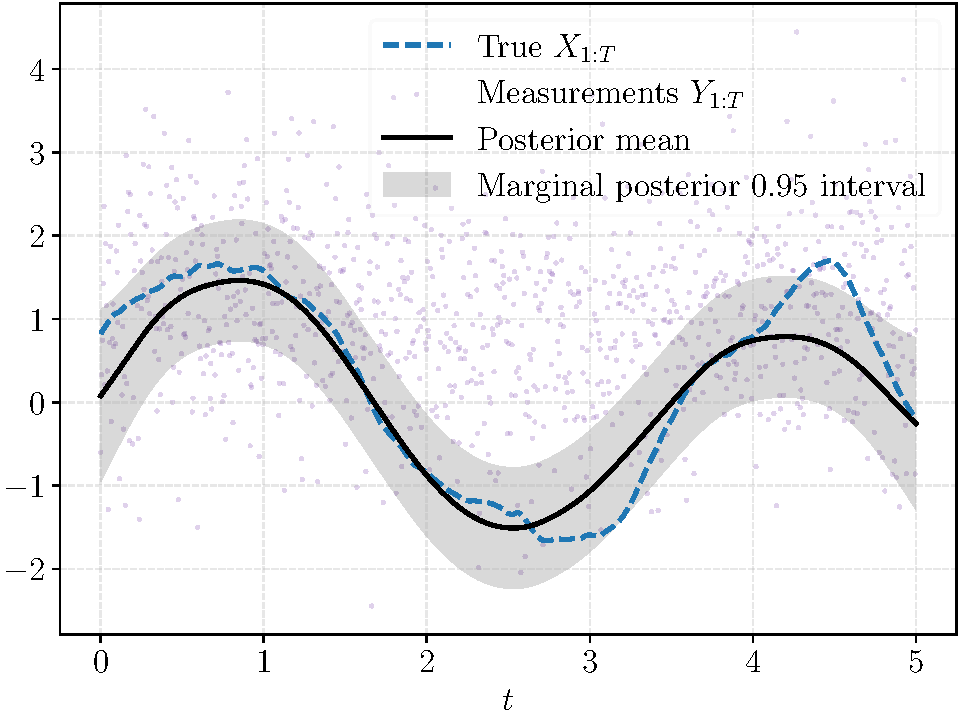
\includegraphics[width=.6\linewidth]{figs/regression}
	\caption{GP regression when $m(t) = \sin(2 \, t)$ and $C$ is a Mat\'{e}rn $\nu=3 \, / \, 2$ covariance function with $\ell=1$ and $\sigma=1$. The model parameters are $a=0.2$, $b=1$, and $\Xi=1$.}
	\label{fig:regression}
\end{figure}

\section{Maximum likelihood estimation of parameters}
Let us recall the GP regression model
%
\begin{equation}
	\begin{split}
		X(t) &\sim \GP\bigl( m(t; \theta), C(t, t'; \theta) \bigr), \\
		Y_k &= a \, X(t_k) + b + \xi_k,
		\label{equ:gp-para-est}
	\end{split}
\end{equation}
and in addition we assume that the GP has an unknown parameter $\theta$ that we want to estimate from the measurements $y_{1:T}$. For instance, in the Mat\'{e}rn case, we can denote $\theta = \begin{bmatrix} \theta_1 & \theta_2 \end{bmatrix}$, and let $\ell = g(\theta_1)$ and $\sigma = g(\theta_2)$ for some positive bijection $g$. To estimate the parameter $\theta$, we commonly use the maximum likelihood estimation (MLE) method. This method consists in maximising the marginal log likelihood
%
\begin{equation*}
	\begin{split}
		\log p(y_{1:T}; \theta) &= \log \int p(y_{1:T} \cond x_{1:T}) \, p(x_{1:T}; \theta) \diff x_{1:T} \\
		&= \log \int \mathrm{N}(y_{1:T} \cond a \, x_{1:T} + b, \Xi \, I_T) \, \mathrm{N}(x_{1:T} \cond m_{1:T}, C_{1:T}; \theta) \diff x_{1:T} \\
		&= -\frac{1}{2} \Bigl(\bigl(y_{1:T} - (a \, m_{1:T} + b)\bigr)^\trans \, G_{1:T}^{-1} \, \bigl(y_{1:T} - (a \, m_{1:T} + b)\bigr) \\
		&\qquad\quad+ \log \det(2 \, \pi \, G_{1:T})\Bigr),
	\end{split}
\end{equation*}
%
with respect to the parameter $\theta$. Please note that now $m_{1:T}$ and $G_{1:T}$ depend on the parameter $\theta$, hence, to find the optimal parameters we have to resort to non-linear optimisers~\citep{Nocedal2006} depending on the mean and covariance functions of the model. The optimisation usually requires the gradient $\partial \log p(y_{1:T}; \theta) \, / \, \partial \theta$. Although you can derive the gradient by hand (this is an exercise), in practice we can compute the gradient efficiently and bug-lessly by using automatic differentiations, for instance, JAX (Python).

We give a demonstration as follows. Let us define a GP model with mean function $m(t;w) = w \sin(\pi \, t)$ and a Mat\'{e}rn $\nu=3  \, / \, 2$ covariance function. Choose $w = 2$, and the length scale and magnitude of the covariance function be $\ell=\sigma=1$. Since it is not possible to identify $a$ and $\sigma$ at the same time, we fix $a=1$ and $b=0$. To minimise the negative log likelihood, we use the L-BFGS-B optimiser. The result is plotted in Figure~\ref{fig:param-mle}. In this figure, we find that the estimated parameters are close to the true ones. 

\begin{figure}[t!]
	\centering
	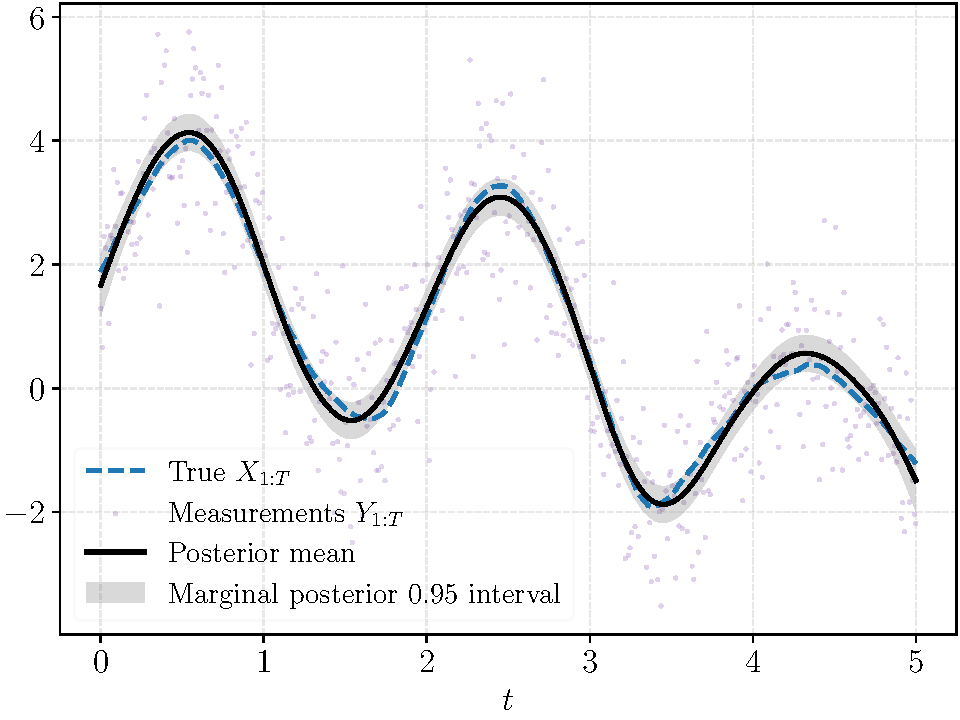
\includegraphics[width=.8\linewidth]{figs/param-mle}
	\caption{The estimated parameters are $w\approx 1.98$, $\sigma \approx 1.33$, and $\ell\approx 1.28$ which are close to the true values $2$, $1$, and $1$, respectively.}
	\label{fig:param-mle}
\end{figure}

\begin{exercise}
	Choose $m(t;w) = \sin(w \, \pi \, t)$ for some $w$, and a Mat\'{e}rn covariance function the same as in Figure~\ref{fig:param-mle}. Try if you can simultaneously estimate $\ell$, $\sigma$, and in particular, $w$, from the data. If not, find out why.
\end{exercise}

\section{Approximate GP regression for non-Gaussian likelihood}
\label{sec:approximate-gp-regression}
In reality many likelihood models (i.e., $p(y_{1:T} \cond x_{1:T})$) are not linear Gaussian like in Equation~\eqref{equ:gp-regression-model}. For example, when use GP for classifications, we often choose a categorical distribution parametrised by the GP through a softmax function. It is hard to solve the posterior distribution of the GP in closed-form.

Textbook methods for approximating the GP posterior distribution include, for example, Laplace approximation and Markov chain Monte Carlo (MCMC). The essence of Laplace approximation is to approximate the GP posterior distribution by a Gaussian whose mean and covariance are given by the maximum a posteriori (MAP) solution, and the inverse Hessian of the MAP, respectively. The Laplace method is a fine example for pedagogy, as it is easy to implement. In the following example, we show a Laplace approximation to a GP regression problem with non-linear Poisson likelihood.

\begin{example}[GP regression with Poisson likelihood]
	\label{example:gp-poisson}
	Consider a GP regression model defined by
	\begin{equation*}
		\begin{split}
			X(t) &\sim \GP\bigl(0, C(t, s)\bigr), \\
			Y_k \cond X(t_k) &\sim \mathrm{Poisson}\bigl(y; \lambda(X(t_k))\bigr),\\
			\lambda(x) &\coloneqq \tanh(x) + 1,
		\end{split}
	\end{equation*}
	where $C$ is an exponential covariance function. The posterior distribution of $X$ in this example is not available in closed-form. In Figure~\ref{fig:poisson-gp} we demonstrate a Laplace approximation to the posterior distribution.
	\begin{figure}[t!]
		\centering
		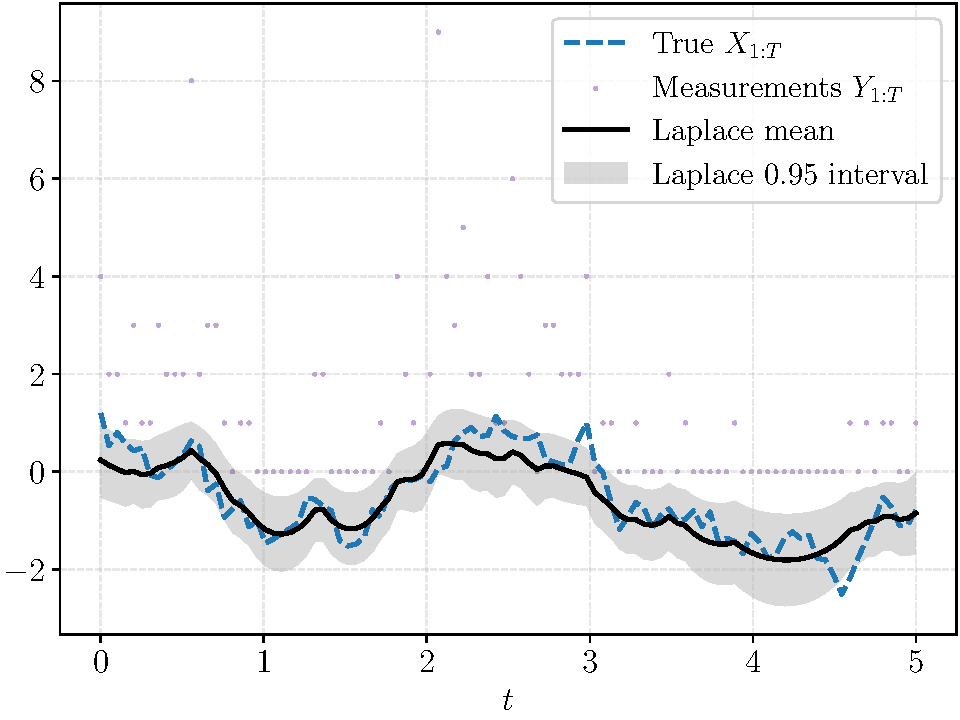
\includegraphics[width=.8\linewidth]{figs/poisson-gp}
		\caption{Laplace approximation to the GP regression model in Example~\ref{example:gp-poisson}.}
		\label{fig:poisson-gp}
	\end{figure}
\end{example}

The bottleneck for GP regression problems is the computation. As an example, when using the Laplace approximation, we need to take a matrix inversion of a Hessian matrix of size $T$. This computation is expensive when $T$ is large. As for the MCMC methods, many of them do not scale well with large $T$ either, because the dimension of the sampling problem is determined by $T$.

We will expand this section in a future version of this lecture note.

Previously in Section~\ref{sec:gp-sampling} we have shown a few methods that can make samples from GP efficiently. These methods in principle may apply to the regression problem as well, but they may introduce approximations even for the linear Gaussian likelihood models, for example, the truncated KKL expansion. In the following section, we briefly sketch two alternative constructions of (Markov) GPs. These GPs can reduce the cubic complexity $O(T^3)$ to a linear one $O(T)$ (even sublinear $O(\log T)$ if implemented in parallel).

\section{Alternative GP constructions for scalability}
\label{sec:gp-markov}
The definition of GP implies that the mean and covariance functions uniquely determine a GP. However, this does not mean that we have to explicitly assign the mean and covariance functions in order to construct a GP. As an example, Brownian motion is a GP by definition, but the definition itself does not explicitly involve its covariance function. Avoiding using the covariance function can be beneficial in computation for large datasets, since we do not need to deal with huge covariance matrices.

In what follows, we briefly recall two commonly used representations of GPs that are scalable for large number of data points. These GPs are called Markov Gaussian processes, and they are computationally efficient thanks to their Markov property. The Markov property is useful because to compute expectations that depend on the entire history, like $\expec{X(t_k) \cond X(t_{k-1}), X(t_{k-2}), \allowbreak\ldots, X(t_0)}$, we only need to condition on the previous one $\expec{X(t_k) \cond X(t_{k-1})}$.


\subsection{Gauss--Markov random fields using precision matrices}
Recall that the computation bottleneck of GP is storing and computing the covariance matrix $C_{1:T}$, and the inversion of $C_{1:T}$. The essence of the Gauss--Markov random field (GMRF) approach consists in representing GPs with the precision matrix instead of the covariance matrix~\citep{Rue2005}. The precision matrix is defined as the inverse of the covariance matrix and can be computed directly from a correlation graph~\citep[see, e.g.,][Thm. 2.3]{Rue2005}. Moreover, thanks to the Markov property of GMRF, the precision matrices of GMRFs are tridiagonal which are sparse. Hence, the storage and algebraic operations (e.g., solving linear systems and spectral decompositions) on the precision matrix are computationally cheap.

\subsection{Linear stochastic differential equations}
\label{sec:sde-gp}
Consider a linear stochastic differential equation (SDE)
%
\begin{equation}
	\diff X(t) = \mu \, X(t) \diff t + \eta \diff B(t), \quad X(t_0) = X_0,
	\label{equ:linear-sde}
\end{equation}
%
where $B$ is a Brownian motion. Solutions to the SDEs of the form in the equation above are continuous-time Markov GPs~\citep[][Sec. 5.6]{Karatzas1991}, and their means and covariance functions are implicitly defined by their SDE coefficients. For details of SDEs, we recommend a course that starts from October 2022 which introduces SDEs from a computational aspect, see \url{https://github.com/spdes/computational-sde-intro-lecture}.

\begin{example}
	\label{example:sde-ou}
	The solution to the SDE
	%
	\begin{equation*}
		\diff X(t) = -\frac{1}{\ell} \, X(t) \diff t + \sqrt{\frac{2}{\ell}} \, \sigma \diff B(t), \quad X(t_0) \sim \mathrm{N}(0, \sigma^2),
	\end{equation*}
	%
	is an exponential/Orstein--Uhlenbeck GP with mean $m(t) = 0$ and the exponential covariance function in Example~\ref{example:ou-gp}. 
\end{example}

There are a number of upsides for using the SDE constructions of GPs. The main upside is computation because we do not need to compute the covariance matrices in, for example, sampling and regression. To make a trajectory from SDE-GPs at times $t_1, t_2, \ldots, t_T$, we can conditionally make samples $X(t_k) \cond X(t_{k-1})$  sequentially in time for $k=1,2,\ldots,T$. This is an algorithm of complexity $O(T)$ which is significantly smaller than the cubic complexity from that of Cholesky decomposition. As for the regression, we can solve the GP posterior distribution of the model in Equation~\eqref{equ:gp-regression-model} by using a Kalman filter and smoother (KFS), and the result from the KFS is exactly the same as from computing Equation~\eqref{equ:gp-posterior}. Computing Equation~\eqref{equ:gp-posterior} requires a cubic complexity, while the complexity of KFS is linear $O(T)$. Moreover, if the KFS is implemented in parallel, the regression problem can be even done faster in logarithmic time~\citep{Corenflos2021SSGP}. We refer the readers to \citet{Sarkka2019} for more details and examples of SDE-GPs.

Another upside of the SDE-GP construction is that many real-world models (e.g., physics and finance) are inherently based on differential equations. For example, in fluid mechanics, we model the motion of fluid, such as velocity and vorticity, by differential equations, since the exact physical solution to the motion are rarely accessible but their infinitesimal dynamics are. When taking randomness into account, these equations become stochastic (partial) differential equations which form (Gaussian) random fields~\citep{Lord2014} under a few assumptions. See, for instance,~\citet{Lindgren2011} for how the SPDE Mat\'{e}rn GPs are applied in geostatistics.

The SDE-GP construction also allows for introducing non-stationarity in a ``simple manner''. As an example, suppose that one desires a Mat\'{e}rn GP such that its length scale and magnitude are some given/learnable functions of time, for instance, $\ell(t) = \mathrm{NN}(t)$ for some (positive) neural networks. In order to do so, one has to invent an extension of the Mat\'{e}rn covariance function, because the original covariance function in Equation~\eqref{equ:matern-cov} will not be a valid covariance function if we just replace its $\ell$ and $\sigma$ by the functions. On the other hand, one can just simply replace these parameters by the desired functions, in the SDE construction of the Mat\'{e}rn GP, for example, in Example~\ref{example:sde-ou}, and the covariance function is automatically valid by definition~\citep[see,][]{Zhao2021Thesis}.

\section{Companion codes}
You may find the implementations of the examples/algorithms of this lecture note at \url{https://github.com/spdes/gp}.

\section{Changelog and errata}

\subsection*{Working release}
\begin{itemize}
	\item Add algebras on covariance functions, and the continuity of GP.
	\item Expand the GP regression for non-linear non-Gaussian likelihood models.
	\item Add examples and materials for the parameter estimation biasedness and identifiability.
\end{itemize}

\subsection*{1 September 2022}
Draft initiated.

\bibliography{refs}
\bibliographystyle{plainnat}

\end{document}
